% =====================================================================
%  Certified Amortized Homogenization
%  Prepared for Computer Methods in Applied Mechanics and Engineering
%  Elsevier elsarticle class, single-column review format.
%
%  Submission metadata must be completed by the authors before submission.
% =====================================================================
\documentclass[preprint,12pt]{elsarticle}

\usepackage{amsmath,amssymb,amsthm,booktabs,graphicx}
\usepackage[colorlinks=true,allcolors=blue]{hyperref}

\newtheorem{theorem}{Theorem}
\newtheorem{proposition}{Proposition}

\journal{Computer Methods in Applied Mechanics and Engineering}

\begin{document}

\begin{frontmatter}

\title{Certified amortized homogenization: guaranteed two-sided bounds on
effective tensors at inference cost}

%% ---------------------------------------------------------------- authors
\author[a]{MD Haffiz Mahamud}
\author[a]{Second author to be confirmed}
\address[a]{Rajshahi University of Engineering \& Technology (RUET), Rajshahi, Bangladesh}

%% ---------------------------------------------------------------- abstract
\begin{abstract}
Computational homogenization returns effective properties without error
bars, while variational bounds return certified intervals but require a
separate solve for every microstructure. Amortized neural surrogates remove
that cost but not the missing guarantee. We combine the two. Primal and
dual trial fields are conditioned on the microstructure so that a single
trained operator emits certified two-sided L\"owner bounds for
microstructures it has never seen. On the controlled numerical
configurations reported here, inference takes 19\,ms for scalar conductivity
and 62\,ms for plane-strain elasticity. The certificate is valid for every
input satisfying the stated discretisation and positive-definiteness
assumptions; training quality affects tightness rather than validity.
On controlled, synthetic periodic test cells, the reported intervals are two
to four times narrower than the Voigt--Reuss envelope. In scalar
conductivity, they also distinguish microstructures that the envelope
cannot---a laminate and a checkerboard of identical phase fraction receive
certified widths of 18.3\% and 43.2\%. We extend the construction to
tensor-valued elasticity using Airy potentials certified on $C^1$
Bogner--Fox--Schmit elements, and demonstrate that construction on synthetic
plane-strain two-phase cells. In illustrative fixed-budget synthetic design
calculations, certified performance floors increase by 55.3\% for
conductivity and 36.5\% for directional stiffness. We further give a
computable criterion comparing a trained field's spectral bandwidth against
the quadrature Nyquist limit, evaluated here as an empirical, label-free
diagnostic for collocation under-resolution. Certified widths and their
limits are mapped across phase contrast and controlled morphology classes,
including a segmented sandstone geometry for scalar conductivity.
A fixed public $200$-cell plane-strain audit gives $200/200$ L\"owner
coverage after an explicit raster-to-Cartesian tensor-coordinate conversion,
independently checked on three cells by periodic $Q_1$ solves. Its median
relative width is $160.9\%$, however, so this external result establishes
coverage rather than competitive tightness.
\end{abstract}

%% ---------------------------------------------------------------- highlights
\begin{highlights}
\item Certified two-sided bounds for unseen controlled-model microstructures in under 100 ms
\item Validity is independent of training quality under the stated certification contract
\item Scalar-conductivity certificates 2-4x tighter than Voigt-Reuss and sensitive to geometry
\item C1 Bogner-Fox-Schmit Airy potentials certify the elastic lower bound
\item Public 200-cell elastic audit: 100\% coverage after coordinate-frame verification
\item A bandwidth-Nyquist test predicts collocation overfitting before it bites
\end{highlights}

\begin{keyword}
computational homogenization \sep guaranteed bounds \sep
physics-informed neural networks \sep operator learning \sep
effective properties \sep certified design
\end{keyword}

\end{frontmatter}

%% ---------------------------------------------------------------- body
% =====================================================================
%  SECTION 1 — Introduction
%  Draft 1. Written LAST and written against sec11_limitations.tex:
%  every claim here is one that section 11 permits.
% =====================================================================

\section{Introduction}
\label{sec:intro}

Effective properties of heterogeneous materials are computed constantly and
certified rarely. A designer screening candidate microstructures, a
qualification engineer justifying an allowable, and an uncertainty study
propagating microstructural variability all need a number for the effective
conductivity or stiffness of a given arrangement of phases. Established
computational homogenization---finite elements, or the FFT schemes of
Moulinec and Suquet~\cite{Moulinec1998}, supplies that number quickly and
accurately. What it does not supply is an error bar: the output is an
estimate whose distance from the exact effective tensor is unknown without
a separate convergence study, and in our own measurements an FFT solve
returned an estimate $3.867\%$ from the analytic value with nothing in its
output to reveal the discrepancy.

Variational bounds resolve this. The primal and complementary energy
principles bracket the effective tensor between two computable matrices,
and the width of the bracket is itself a certificate of accuracy. The
construction dates to the hypercircle method of Prager and
Synge~\cite{PragerSynge1947} and has been developed into guaranteed
computable bounds for homogenization by several
groups~\cite{Vondrejc2015,Vondrejc2016,Gaynutdinova2023}.
Its neural realisation is recent: Gaynutdinova et
al.~\cite{Gaynutdinova2026} train primal and dual networks for the scalar
conductivity cell problem and certify the resulting bounds by projecting
the networks onto conforming piecewise-linear finite elements, where the
energy integrals can be evaluated exactly. Their formulation is, however,
per-instance: every microstructure requires its own training run, which is
precisely the wrong cost model for the many-query settings above.

Machine-learned surrogates address the cost. Amortized homogenization is by
now well established: graph networks that take the microstructure as an
input and generalise to geometries absent from training~\cite{Hendriks2024},
physics-informed solvers of the cell problem with architecturally enforced
periodicity~\cite{Jiang2023}, and label-free energy-minimising neural
solvers for periodic microstructures~\cite{Xing2025}. Most such approaches
report estimates rather than a geometry-specific computable error bound.
A notable exception is the Voigt--Reuss network of Keshav, Herb and
Fritzen~\cite{Keshav2025}, which predicts stiffness tensors
for unseen microstructures and enforces, by construction, that every
prediction lies inside the analytic Voigt--Reuss envelope in the L\"owner
sense. That envelope, however, is a function of the phase fractions alone:
it assigns the same admissible set to every composite of the same
composition, and therefore certifies physical admissibility rather than
per-instance accuracy.

\medskip
The three positions may be summarised as follows.

\begin{center}
\resizebox{\textwidth}{!}{%
\begin{tabular}{lll}
\toprule
 & certificate & scope \\
\midrule
Gaynutdinova et al.~\cite{Gaynutdinova2026} & variational, tight & per-instance, scalar \\
Voigt--Reuss net~\cite{Keshav2025} & amortized, fraction-only & tensor elasticity \\
\textbf{this work} & \textbf{amortized and per-instance tight} & scalar and tensor, 2D \\
\bottomrule
\end{tabular}}
\end{center}
\medskip

This paper occupies the missing entry. We stress the precise claim:
amortization over unseen microstructures is not itself new~\cite{Hendriks2024,Jiang2023,Xing2025},
and exact-integration certification of neural trial fields is not
new~\cite{Gaynutdinova2026}. Our contribution is their combination,
\emph{certified} amortization: two-sided bounds for microstructures not
used to train the operator, computed at inference cost, under the
certification contract stated below. The results demonstrate tighter
intervals than the analytic envelope on the reported test cases; they do
not establish superiority to every certified or learned competitor.

\subsection{Contributions}

\paragraph{Certified amortization.} We condition primal and dual trial
fields on the microstructure in a way that preserves conformity, so that a
single trained operator emits certified bounds for unseen microstructures.
The reported inference timings, $19$\,ms for conductivity and $62$\,ms for
elasticity, are measured on the controlled generated families used here.
Unlike amortized
surrogates that regress the effective tensor
directly~\cite{Hendriks2024,Keshav2025}, the operator here emits
\emph{admissible fields}, from which the bounds follow by the variational
principles of Section~\ref{sec:primaldual}; the guarantee is therefore a
property of the construction rather than of the training data. Under the
certification contract, the bound theorems hold for every input whether or
not it resembles the training distribution. The interval width is a
geometry-specific measure of trial-field suboptimality, not a universal
detector of distribution shift. We show that this conditioning must be
smooth and periodic
within the automatic-differentiation graph---the natural implementation
using per-point coefficient lookups destroys conformity and voids the
guarantee---a constraint that cannot arise in per-instance formulations.

\paragraph{Certificates that see geometry.} On the controlled scalar
conductivity test cells, certified intervals are between two and four times
narrower than the Voigt--Reuss envelope. More directly, for two
microstructures of identical phase fraction $0.500$, a rank-one laminate and
a checkerboard, the envelope is by construction the same, while the
certified widths are $18.3\%$ and $43.2\%$ respectively. A guarantee
derived from composition cannot make this distinction; a variational
certificate does, at inference cost.

\paragraph{Tensor-valued elasticity.} We extend the amortized construction
to plane-strain elasticity, representing statically admissible periodic
stresses through Airy potentials and certifying them by projection onto
$C^1$ Bogner--Fox--Schmit elements, where global $C^1$ continuity is
exactly what makes the interpolated traction continuous across element
edges. The classical form of this dual is due to Gaynutdinova et
al.~\cite{Gaynutdinova2023}; the contribution here is carrying it onto
amortized neural trial fields with exact-integration certification.

\paragraph{A criterion for collocation adequacy.} That a
collocation-evaluated loss can be arbitrarily misleading is
known~\cite{Berrone2022}, and integration overfitting has been observed
empirically in this
setting~\cite{Gaynutdinova2026}. We contribute prediction and prescription:
a computable comparison between the trained field's spectral bandwidth and
the Nyquist limit of the quadrature rule that flags the failure before
certification degrades, functions as a per-run and label-free accept/reject
gate, and motivates how to choose the collocation density. In the reported
experiments, bandwidth exceeding the Nyquist limit accompanied inaccurate
collocation energies, including reported upper bounds below the analytic
reference. We treat the diagnostic as empirical; it is not a universal
acceptance criterion for physics-informed networks.

\paragraph{Applications.} Because the certificate is differentiable, the
design objective can be the guaranteed value itself. In illustrative
fixed-budget synthetic calculations, optimising inclusion positions raises a
guaranteed conductivity floor by $55.3\%$ and a guaranteed directional
stiffness floor by $36.5\%$.
The construction is self-penalising: a looser dual field yields a lower guaranteed floor, so the optimiser cannot profit from degrading the
surrogate, which is the failure mode that makes surrogate-driven design
untrustworthy. Separately, for the same specified geometry, phase law,
boundary conditions, tensor convention and discretisation, a reference value
falling outside the interval establishes an inconsistency that must be
resolved; we report a case in which the certificate identified an
under-converged finite-volume solution, confirmed subsequently by mesh
refinement.

\paragraph{Intended use.} We state at the outset the regime each mode
serves, since the certified widths differ by an order of magnitude between
them. In the synthetic elasticity experiment, amortized certificates had a
median width of $28\%$ and are intended for \emph{screening}: a requirement falling outside the interval
decides a candidate provably, and Section~\ref{sec:amortized:screening}
shows that this settles roughly two thirds of a design pool at $10$\,ms per
candidate. Per-instance certification, reaching widths below $1\%$, is
intended for final design. We do not claim that a $28\%$ interval is a
design-grade property estimate.

\subsection{Scope}

We state the boundaries here rather than only in
Section~\ref{sec:limitations}. The construction is two-dimensional, linear
and periodic, and excludes voids and rigid phases. In the controlled
families studied here, certified widths degrade towards the analytic envelope
for corner-singular and bicontinuous morphologies above roughly $50{:}1$
phase contrast; we map this boundary explicitly rather than reporting only
favourable cases, and identify the limitation as the approximation of
complex corrector fields by smooth networks rather than any failure of the
certification machinery. We claim
no speed advantage over classical homogenization. An FFT solve of these cells is roughly fifty times faster per query, and the amortized route
becomes preferable only beyond approximately $300$ certified queries. Nor
do we claim experimental validation: the certificate concerns a specified
idealised periodic model and is validated here against closed-form effective
tensors and independent finite-volume, finite-element and FFT calculations
for matching model problems. The reported plane-strain performance results
are otherwise controlled numerical demonstrations on author-generated
periodic two-phase cells. We additionally report a fixed external coverage
audit on $200$ labelled cells from the public DaRUS-5730 plane-strain
dataset~\cite{Keshav2026data}. It uses the released native $100\times100$
rasters, an explicit image/tensor coordinate-frame conversion, and the
released phase law; the latter conversion is independently checked by
periodic $Q_1$ calculations on three formerly discrepant cells. We do not,
however, report a head-to-head trained-predictor comparison. Such a
comparison requires the same fixed split and a documented match of geometry,
phase law, boundary condition, tensor convention and discretisation.

\subsection{Outline}

Section~\ref{sec:primaldual} states the primal--dual certificates and fixes
notation. Section~\ref{sec:admissible} describes how admissibility is
enforced by architecture, and Section~\ref{sec:exact} how the certificates
are made exact by projection onto conforming finite elements.
Section~\ref{sec:amortized} presents the amortized construction and its
results, and Section~\ref{sec:tightness} compares the resulting
certificates against the analytic envelope. Section~\ref{sec:quadrature}
develops the collocation-adequacy criterion, and Section~\ref{sec:limits}
maps the boundary of usefulness across contrast and morphology.
Sections~\ref{sec:applications} and~\ref{sec:cost} give applications and an
honest cost comparison, and Section~\ref{sec:limitations} collects the
limitations.

% =====================================================================
%  SECTIONS 2-4 — Certificates, architectural admissibility, exact
%  integration. Draft 1.
% =====================================================================

\section{Primal--dual certificates}
\label{sec:primaldual}

Let $Y = [0,1)^2$ be the unit cell, $k \in L^\infty(Y)$ a positive
piecewise-constant coefficient, and $\langle \cdot \rangle$ the average over
$Y$. For a prescribed mean gradient $\bar g$ the corrector $\theta$ solves
$\operatorname{div}\!\big(k(\bar g + \nabla\theta)\big) = 0$ with $\theta$
$Y$-periodic, and the effective tensor admits the variational
characterisation~\cite{Milton2002}
%
\begin{equation}
  \bar g \cdot K_{\mathrm{eff}}\, \bar g
  \;=\; \min_{\theta \in H^1_{\mathrm{per}}(Y)}
  \big\langle (\bar g + \nabla\theta) \cdot k (\bar g + \nabla\theta) \big\rangle .
  \label{eq:primal}
\end{equation}

\subsection{Upper bound}

\begin{theorem}[Primal certificate]
\label{thm:primal}
Let $\chi_1,\chi_2 \in H^1_{\mathrm{per}}(Y)$ be arbitrary and set
$G_i = e_i + \nabla \chi_i$. Then
%
\begin{equation}
  \big[K_{\mathrm{up}}\big]_{ij} := \big\langle k\, G_i \cdot G_j \big\rangle
  \qquad \text{satisfies} \qquad
  K_{\mathrm{up}} \;\succeq\; K_{\mathrm{eff}}
  \label{eq:Kup}
\end{equation}
%
in the L\"owner order.
\end{theorem}

\begin{proof}
Take the load-linear trial family
$\theta(\bar g) = \bar g_1 \chi_1 + \bar g_2 \chi_2$, which is admissible
in~\eqref{eq:primal} for every $\bar g$. Substituting gives
$\bar g \cdot K_{\mathrm{eff}} \bar g \le \bar g^{\!\top} K_{\mathrm{up}} \bar g$
for all $\bar g$, which is the assertion.
\end{proof}
Linearity of the trial map in $\bar g$ is the only structural requirement,
which is why the construction uses one field per unit load and combines
loads by superposition rather than supplying $\bar g$ as a network input.

\subsection{Lower bound}

The complementary principle characterises the inverse,
%
\begin{equation}
  \bar q \cdot K_{\mathrm{eff}}^{-1} \bar q
  \;=\; \min_{\substack{\operatorname{div} q = 0 \\ \langle q \rangle = \bar q}}
  \big\langle q \cdot k^{-1} q \big\rangle .
  \label{eq:dual}
\end{equation}
%
\begin{theorem}[Dual certificate]
\label{thm:dual}
Let $Q_i$ be admissible in~\eqref{eq:dual} with $\langle Q_i \rangle = e_i$.
Then $S_{\mathrm{up}} := \big[\langle k^{-1} Q_i \cdot Q_j\rangle\big]
\succeq K_{\mathrm{eff}}^{-1}$ and consequently
%
\begin{equation}
  K_{\mathrm{low}} := S_{\mathrm{up}}^{-1} \;\preceq\; K_{\mathrm{eff}}
  \;\preceq\; K_{\mathrm{up}} .
  \label{eq:sandwich}
\end{equation}
\end{theorem}

\begin{proof}
The superposition argument of Theorem~\ref{thm:primal} applied
to~\eqref{eq:dual} gives $S_{\mathrm{up}} \succeq K_{\mathrm{eff}}^{-1}$;
inversion reverses the L\"owner order on symmetric positive definite
matrices, and the upper bound is Theorem~\ref{thm:primal}.
\end{proof}

The width of~\eqref{eq:sandwich} is a computable per-instance error
certificate. The construction is classical: it is the hypercircle
argument of Prager and Synge~\cite{PragerSynge1947}, developed for
homogenization by Dvo\v{r}\'ak and Haslinger and realised with exact
integration in a Fourier--Galerkin setting by Vond\v{r}ejc and
co-workers~\cite{Vondrejc2015,Vondrejc2016}, and with guaranteed two-sided
stiffness bounds by Gaynutdinova et al.~\cite{Gaynutdinova2023}. Its neural realisation for
scalar conductivity, including certification by projection onto conforming
finite elements, is due to Gaynutdinova et al.~\cite{Gaynutdinova2026}.
Our contribution begins after this point.

We distinguish this construction from the broader literature on computable
error bounds for physics-informed networks, which certifies a \emph{field}
rather than a homogenized tensor: certified wavelet-based
approximations with computable upper bounds~\cite{Ernst2024}. Such results bound the
distance between a network and the solution of a PDE. The certificates here
bound a \emph{functional} of that solution, the effective tensor, from two sides, and do so without any stability or coercivity constant entering
the estimate, because the bounds follow from minimisation rather than from
residual propagation.

\subsection{Elasticity}

In Mandel notation, where strains and stresses are represented as
$(\varepsilon_{11}, \varepsilon_{22}, \sqrt{2}\,\varepsilon_{12})$ and
$(\sigma_{11}, \sigma_{22}, \sqrt{2}\,\sigma_{12})$, the L\"owner order on
stiffness matrices is literal matrix ordering and the compliance is a plain
matrix inverse. With three unit Mandel strains $E_k$ and total strains
$F_k = E_k + \varepsilon(\chi_k)$, and three unit Mandel stresses $T_k$
with statically admissible total stresses $\Sigma_k$,
%
\begin{equation}
  \big[C_{\mathrm{up}}\big]_{kl} = \langle F_k \cdot \mathbb{C} F_l \rangle
  \succeq C_{\mathrm{eff}}, \qquad
  \big[S_{\mathrm{up}}\big]_{kl} = \langle \Sigma_k \cdot \mathbb{S} \Sigma_l \rangle,
  \quad C_{\mathrm{low}} = S_{\mathrm{up}}^{-1} \preceq C_{\mathrm{eff}} .
  \label{eq:elastic}
\end{equation}

\section{Admissibility by architecture}
\label{sec:admissible}

The bounds~\eqref{eq:sandwich} and~\eqref{eq:elastic} hold for
\emph{any} admissible fields. We therefore enforce admissibility
structurally, so that optimisation quality affects tightness rather than
validity. A poorly trained model need not be reliably identified by a wide
interval, but its projected and exactly integrated output remains a valid
certificate whenever the following contract is met.

\paragraph{Periodicity.} Networks receive only the Fourier features
$\{\sin 2\pi m y_c, \cos 2\pi m y_c\}_{m \le M,\, c=1,2}$. Any smooth
function of these is $Y$-periodic, and the mean of the gradient of a
periodic field vanishes identically.

\paragraph{Primal fields.} One scalar head per unit load (two for
conductivity, six for plane-strain elasticity: three loads times two
displacement components) supplies $\chi_i$ directly; the trial family is
linear in the load by construction, as~\eqref{eq:Kup} requires.

\paragraph{Scalar dual.} Writing the flux fluctuation as the rotated
gradient of a periodic stream function,
$q = \bar q + \operatorname{curl}\psi$ with
$\operatorname{curl}\psi = (\partial_2 \psi, -\partial_1 \psi)$, gives
$\operatorname{div} q = \psi_{,21} - \psi_{,12} = 0$ identically and
$\langle \operatorname{curl}\psi\rangle = 0$ exactly. Both constraints
of~\eqref{eq:dual} are thus satisfied by construction rather than by
penalty. This is the construction of~\cite{Gaynutdinova2026}.

\paragraph{Tensor dual.} In two dimensions the Airy representation
%
\begin{equation}
  \sigma'_{11} = \varphi_{,22}, \qquad
  \sigma'_{22} = \varphi_{,11}, \qquad
  \sigma'_{12} = -\varphi_{,12}
  \label{eq:airy}
\end{equation}
%
is symmetric, divergence-free identically, and has exactly zero mean for
periodic $\varphi$, since the mean of any second derivative of a periodic
field vanishes. Three potentials, one per unit Mandel stress, therefore
give statically admissible $\Sigma_k$ with exactly the prescribed means.
The corresponding classical construction, a self-equilibrated stress field
generated from a stress potential and discretised with $C^1$
Bogner--Fox--Schmit elements, is due to Gaynutdinova et
al.~\cite{Gaynutdinova2023}; we carry it onto neural trial fields.

\paragraph{Initialisation.} Zero-initialising the output layers makes the
trial fluctuations vanish, so the certificate at step zero is exactly the
Voigt--Reuss envelope (Figure~\ref{fig:convergence}): $K_{\mathrm{up}} = \langle k \rangle I$ and
$K_{\mathrm{low}} = \langle k^{-1}\rangle^{-1} I$. Validity therefore holds
from the first iteration and training can only tighten.

\begin{figure}[t]
\centering
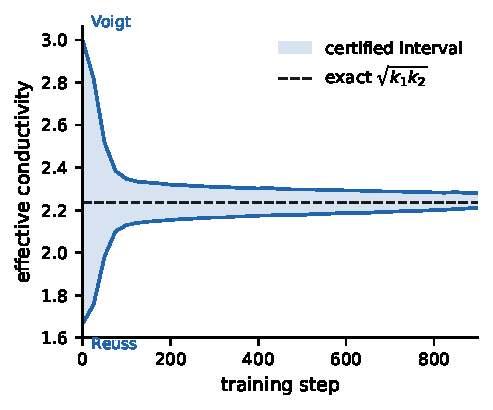
\includegraphics[width=0.62\linewidth]{figures/fig_convergence.pdf}
\caption{Certified bounds closing from the Voigt--Reuss envelope onto the
exact effective conductivity of a two-phase checkerboard. Zero-initialised
output layers make the first iterate exactly the classical envelope, and
every subsequent iterate is a valid certificate; training tightens the
interval but is not required for validity.}
\label{fig:convergence}
\end{figure}

\paragraph{Objective.} Since each head appears in exactly one term of
$\operatorname{tr} K_{\mathrm{up}} + \operatorname{tr} S_{\mathrm{up}}$ and
is minimised by the corresponding true corrector, minimising this sum
tightens both bounds simultaneously. No reference solutions enter training;
finite-element and FFT solvers are used only to audit the implementation.

\section{Exact-integration certification}
\label{sec:exact}

The bounds are statements about integrals, and a scheme that evaluates them
by sampling inherits the quadrature error, which Section~\ref{sec:quadrature} shows can be severe enough to invalidate a
certificate. We remove the dependence entirely by interpolating the trained
fields into conforming finite-element spaces on a mesh aligned with the
phase boundaries and integrating exactly. The network proposes; the
projection certifies.

\paragraph{Primal.} Nodal $Q_1$ interpolation of a continuous periodic
field is continuous, piecewise bilinear and periodic, hence lies in a
conforming subspace of $H^1_{\mathrm{per}}$, and~\eqref{eq:Kup} applies
verbatim.

\paragraph{Scalar dual.} Let $\psi_h$ be continuous piecewise bilinear and
$q = \operatorname{curl}\psi_h$. Within each element
$\operatorname{div} q = 0$ pointwise. Across an element edge, continuity of
$\psi_h$ forces its \emph{tangential} derivative to be continuous, and the
curl rotates tangential into normal, so the \emph{normal} component of $q$
is continuous, which is precisely the condition for $q \in H(\operatorname{div})$
with vanishing divergence. Interpolation therefore certifies the dual side
with no need for $H(\operatorname{div})$-conforming elements.

\paragraph{Tensor dual.} The $Q_1$ space cannot carry an Airy stress, since
bilinear functions have $\varphi_{,11} = \varphi_{,22} = 0$ identically. We
use the Bogner--Fox--Schmit bicubic Hermite space, with nodal degrees of
freedom $(\varphi, \varphi_{,x}, \varphi_{,y}, \varphi_{,xy})$, all four
obtained exactly by automatic differentiation of the network. Global $C^1$
continuity is what makes the interpolated stress admissible: across an edge
with normal $e_1$ the traction components are
$(\varphi_{,22}, -\varphi_{,12})$; $\varphi_{,22}$ is a second tangential
derivative of a continuous function, and $\varphi_{,12}$ is the tangential
derivative of $\varphi_{,1}$, which is continuous by $C^1$ regularity.
Traction is therefore continuous, the interpolated stress lies in
$H(\operatorname{div})$ with vanishing divergence, and its cell mean is
exact.

\paragraph{Exactness of the quadrature.} On a phase-aligned mesh the
coefficient is constant per element. Gradients of $Q_1$ fields are
bilinear, so the primal integrand has degree at most two per coordinate and
$2\times 2$ Gauss is exact. Second derivatives of BFS fields have degree at
most three per coordinate, so the complementary integrand has degree at
most six and $4 \times 4$ Gauss, exact to degree seven, suffices. The
resulting certificates hold up to floating-point arithmetic only.

\begin{proposition}[Certification contract]
\label{prop:contract}
For each reported input, the bounds in \eqref{eq:sandwich} and
\eqref{eq:elastic} are certified for the discretised periodic problem if:
(i) every phase coefficient is uniformly positive definite; (ii) the
certification mesh resolves every phase boundary, so the coefficient is
constant on each element; (iii) the projected primal fields are periodic
and belong to the stated conforming $H^1$ spaces; (iv) the projected dual
fields have the prescribed cell means and belong to $H(\operatorname{div})$
with zero divergence; and (v) the stated elementwise Gauss rules are used.
The conclusion is subject only to floating-point round-off.
\end{proposition}

\begin{proof}
Conditions (iii) and (iv) make the primal and complementary trial fields
admissible in the variational principles. Theorems~\ref{thm:primal} and
\ref{thm:dual}, and their elasticity analogues, then give the L\"owner
ordering. Conditions (i), (ii), and (v) ensure that the assembled energy
integrals are the exact finite-element integrals described above.
\end{proof}

\paragraph{Verification.} Table~\ref{tab:anchors} reports the
machine-precision anchors, obtained by feeding closed-form optimal fields
through the production assembly. Because the analytic correctors are
elementwise polynomial, interpolation is exact and any discrepancy would
indicate an implementation error rather than an approximation.

\begin{table}[t]
\centering
\caption{Machine-precision verification. Closed-form optimal fields passed
through the production code path must reproduce the exact effective tensor.}
\label{tab:anchors}
\resizebox{\textwidth}{!}{%
\begin{tabular}{llll}
\toprule
projection & space & anchor & agreement \\
\midrule
scalar primal and dual & $Q_1$ ($C^0$) & rank-one laminate & $10^{-12}$ \\
elasticity primal & $Q_1$ vector & elastic laminate & $10^{-11}$ \\
elasticity dual & BFS bicubic Hermite ($C^1$) & Airy potential of the laminate & $10^{-10}$ \\
\bottomrule
\end{tabular}}
\end{table}

One normalisation deserves record, since it caused an error during
development that the anchors detected. The stress fields associated with
the \emph{strain}-basis solutions have mean stress $C_{\mathrm{eff}}$
rather than the unit basis, so their compliance-weighted Gram matrix is
$C_{\mathrm{eff}}$ itself and inverting it returns
$C_{\mathrm{eff}}^{-1}$. Analytic or imported trial stresses must therefore
be recombined to unit mean, $\Sigma(T_j) = \sum_k [C_{\mathrm{eff}}^{-1}]_{kj}
\sigma^{(k)}$, before entering~\eqref{eq:elastic}. The network path is
immune, its trial means being the unit $T_k$ by construction.

% =====================================================================
%  SECTION 5 — Amortization: certificates for unseen microstructures
%  Draft 1. Every number traceable to RESULTS.md.
% =====================================================================

\section{Amortization: certificates at inference cost}
\label{sec:amortized}

Sections~\ref{sec:admissible}--\ref{sec:exact} produce a certified interval
for \emph{one} microstructure at the cost of one training run. That is the
setting of all existing variational-certificate work, neural or classical:
Gaynutdinova et al.~\cite{Gaynutdinova2026} train one network per
representative cell, and the classical schemes
of~\cite{Gaynutdinova2023} solve one linear system per
cell. For screening, design or uncertainty propagation, the settings in which many-query cost dominates, this is the wrong cost model.

This section removes the per-instance restriction. We condition the trial
fields on the microstructure so that a single trained operator emits
certified bounds for microstructures it has never seen, at inference cost.
The central observation is that this changes nothing about validity:

\begin{proposition}[Certificates survive conditioning]
\label{prop:amortized}
Let $\chi(\,\cdot\,;m)$ and $\psi(\,\cdot\,;m)$ be trial fields
conditioned on a microstructure descriptor $m$, and suppose that for every
fixed $m$ they remain $Y$-periodic and conforming in the sense of
Section~\ref{sec:admissible}. Then the bounds of
Theorems~\ref{thm:primal}--\ref{thm:dual} hold for every $m$, whether or
not $m$ was seen during training.
\end{proposition}

The proof is immediate: admissibility is a property of the fields at fixed
$m$, and the variational arguments never reference the training distribution.
Thus, under the certification contract, out-of-distribution inputs cannot
produce invalid certificates. They need not, however, produce wider
intervals than in-distribution inputs. The interval width is a computable
geometry-specific measure of trial-field suboptimality; it is not an
assumption-free detector of distribution shift or competence.

\subsection{Conditioning that preserves conformity}
\label{sec:amortized:conditioning}

The hypothesis of Proposition~\ref{prop:amortized} is not automatic, and
the natural implementation violates it. Conditioning on per-point lookups
of the phase field, feeding $k(y)$ and its neighbours as network inputs,
produces features that are piecewise constant in $y$. The trial
field then inherits jump discontinuities at phase-cell boundaries, leaves
$H^1$, and its energy bounds nothing. The failure is silent: the code runs,
the numbers look plausible, and the guarantee is gone. This constraint does
not arise in per-instance formulations, where the microstructure enters
only through the coefficient and never through the trial space.

We therefore require conditioning channels that are smooth and periodic in
$y$ \emph{within the automatic-differentiation graph}. Per instance we
project the log coefficient onto low half-plane Fourier modes, blur the
coefficients at two length scales, and evaluate analytically at query time,
%
\begin{equation}
  \tilde k_s(y) \;=\; \bar k \;+\!\! \sum_{\xi \in \mathcal{H}}\!
  e^{-2\pi^2 s^2 |\xi|^2}
  \big( a_\xi \cos 2\pi \xi\!\cdot\! y + b_\xi \sin 2\pi \xi \!\cdot\! y \big),
  \label{eq:conditioning}
\end{equation}
%
supplying $[\tilde k_s(y), \nabla \tilde k_s(y)]_s$ together with global
statistics as conditioning features. Because the trigonometric functions
are evaluated from $y$ in-graph, the resulting fields are $C^\infty$ and
$Y$-periodic in $y$ for every $m$; spatial derivatives remain exact; and
the construction is resolution-agnostic, being defined for any grid finer
than twice the largest retained mode. Zero-initialising the output layers
makes the operator emit exactly the Voigt and Reuss bounds for
\emph{every} instance before training begins, so validity holds from the
first iteration.

\subsection{Conductivity}
\label{sec:amortized:scalar}

A single operator was trained on $40$ random two-phase microstructures at
contrast $10$ ($400$ steps, $123$\,s, one CPU core), with no labels: the
objective is the expected sum of energy and complementary energy over the
family. On eight held-out microstructures the operator produced certified
intervals with mean relative width $28.0\%$ (maximum $40.2\%$) against a
Voigt--Reuss level of $90.1\%$, all eight valid and all bracketing an
independent finite-volume reference, at $19$\,ms per certificate.

The cost comparison against per-instance training on the same instance,
Table~\ref{tab:economics}, is the point of the construction.

\begin{table}[t]
\centering
\caption{Amortization economics, conductivity, identical microstructure.}
\label{tab:economics}
\resizebox{\textwidth}{!}{%
\begin{tabular}{lrr}
\toprule
route & certified width & wall clock \\
\midrule
per-instance training ($400$ steps) & 9.91\% & 25\,s \\
amortized inference & 26.58\% & \textbf{19\,ms} \\
\bottomrule
\end{tabular}}
\end{table}

Figure~\ref{fig:amortization} places this in the many-query setting.
Figure~\ref{fig:tightness-cost} places the trade-off against the
per-instance route at several budgets. Three orders of magnitude in
cost for a factor $2.7$ in width, with
validity never part of the trade. Out of distribution, and audited against
\emph{exact} effective tensors rather than reference solvers, the operator
remained valid on unseen morphology families, with laminates at $12.04\%$ and
$11.65\%$, a corner-singular checkerboard at $39.04\%$---and on a tenfold
contrast extrapolation, where the width grew to $174.64\%$ while the
certificate still contained the exact tensor. The width therefore orders
itself by severity of shift: benign family shift barely widens the
interval, whereas a contrast shift far outside the training range widens it
sixfold and announces itself.


\begin{figure}[t]
\centering
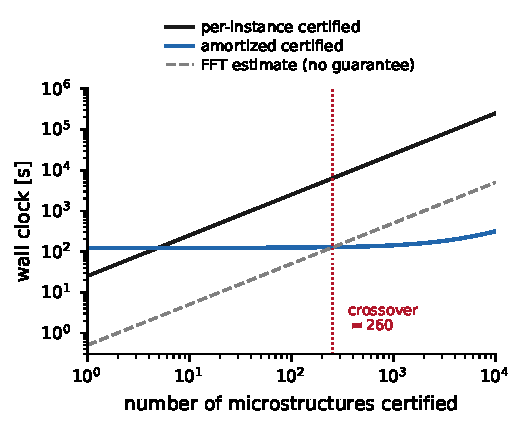
\includegraphics[width=\linewidth]{figures/fig_amortization.pdf}
\caption{Cost to a certified answer. The amortized route overtakes repeated per-instance certification immediately and repeated FFT solves at roughly 300 microstructures, while returning an interval rather than an estimate.}
\label{fig:amortization}
\end{figure}


\begin{figure}[t]
\centering
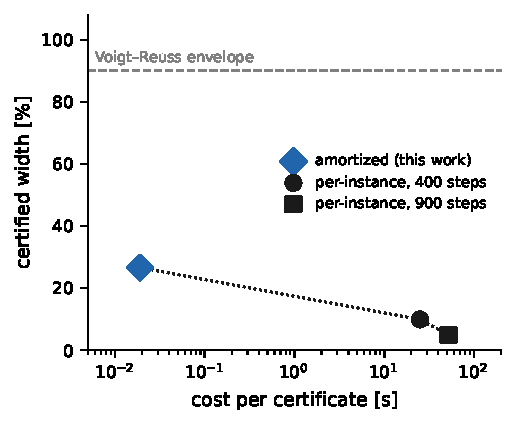
\includegraphics[width=0.62\linewidth]{figures/fig_tightness_cost.pdf}
\caption{Certified width against cost per certificate. Per-instance
training buys tightness at three orders of magnitude more cost per
microstructure; both routes remain far inside the Voigt--Reuss envelope.
A practitioner may choose either, and the amortized route is intended for
screening rather than final design.}
\label{fig:tightness-cost}
\end{figure}

\subsection{Controlled synthetic plane-strain demonstration}
\label{sec:amortized:elastic}

We next exercise the plane-strain construction on a controlled family of
synthetic periodic two-phase cells. With six displacement heads and three
Airy potentials, an operator trained on $200$ generated microstructures for
$4000$ steps in single precision on one GPU ($878$\,s), and certified in
double precision on the CPU by exact integration, produced intervals for
twelve generated held-out cells with median relative width $28.3\%$ (range
$11.2\%$--$45.5\%) at $62$\,ms per certificate. These values quantify
tightness and amortization within this specified generated family; they are
not an externally labelled elasticity coverage study.

For all twelve cells, the projected fields satisfied the certification
contract and the one-sided internal consistency check
$C_{\mathrm{low}} \preceq C_{\mathrm{FEM}}(h)$ held for a conforming $Q_1$
calculation of the same discretised model. This follows from the nested
admissible spaces and checks the implementation path; it is not an
independent validation of the resulting interval against an external
effective-stiffness reference.

\subsection{External public-data coverage audit}
\label{sec:amortized:external}

We next evaluate coverage against the public two-dimensional plane-strain
portion of DaRUS-5730~\cite{Keshav2026data}. The archive provides periodic
binary $100\times100$ rasters and effective stiffness tensors generated by
the Fourier-Accelerated Nodal Solver under periodic boundary conditions. We
retain the released raster without resampling. The released tensor is in an
engineering-Voigt raster frame, whereas the finite-element calculation uses
a right-handed Cartesian frame. We therefore apply the exact Mandel
coordinate transformation $T=\operatorname{diag}(1,1,-1)$ after the usual
Voigt-to-Mandel conversion. This reverses only the normal--shear couplings;
it is a change of coordinates, not a fit or an alteration of a label.

After resolving this coordinate convention by independent $Q_1$ calculations,
we fixed the scaled protocol: $40$ training cells and $40$ validation cells
were selected from each of five Fourier-mode grids, giving $200$ label-free
training cells and $200$ disjoint labelled validation cells. We trained for
$500$ steps and certified every validation cell on the native
$100\times100$ phase-aligned $Q_1$/BFS mesh. The result is reported in
Table~\ref{tab:external-elasticity}.

\begin{table}[t]
\centering
\caption{Fixed external plane-strain coverage audit on DaRUS-5730. Training
uses no reference stiffness tensor. Margins are the smallest eigenvalues of
$C_{\rm ref}-C_{\rm low}$ and $C_{\rm up}-C_{\rm ref}$ in the common
Cartesian Mandel frame.}
\label{tab:external-elasticity}
\resizebox{\textwidth}{!}{%
\begin{tabular}{lr}
\toprule
quantity & result \\
\midrule
training / held-out cells & $200$ / $200$ \\
native raster and certification mesh & $100\times100$ / $100\times100$ \\
reference containment & $200/200$ (100\%) \\
minimum $\lambda_{\min}(C_{\rm ref}-C_{\rm low})$ & $1.264\times10^{-2}$ \\
minimum $\lambda_{\min}(C_{\rm up}-C_{\rm ref})$ & $3.141$ \\
median certified relative width & $160.9\%$ \\
median Voigt--Reuss-width / certified-width & $1.05\times$ \\
independent periodic $Q_1$ checks & $3$ raw-frame failures from this cohort, max. relative tensor error $8.40\times10^{-11}$ \\
\bottomrule
\end{tabular}}
\end{table}

All $200$ transformed reference tensors lie strictly inside the reported
L\"owner intervals. In contrast, comparing the tensor in its raw raster
frame produces $175/200$ containment; that apparent failure is entirely
explained by the sign of the normal--shear couplings. Independent
matrix-free periodic $Q_1$ calculations on three of the cells that fail in
the raw frame reproduce all components of the transformed reference tensor
to relative error at most $8.40\times10^{-11}$. The external certificates
are wide (median $160.9\%$) and only modestly tighter than the analytic
envelope (median $1.05\times$). Thus this experiment validates the
geometry, material law, coordinate convention and coverage contract; it
does not establish competitive external tightness or predictive accuracy.

We report two negative or unexpected results in the interest of an honest
record.

\paragraph{The limit is capacity, not compute.} The monitored gap fell from
$75.4\%$ to $25.3\%$ by step $1200$ and then remained flat through step
$4000$; a smaller run using $40$ microstructures and $450$ steps reached a
held-out median of $28.2\%$, statistically indistinguishable from the
$28.3\%$ obtained with five times the data and nine times the steps.
Table~\ref{tab:ablation} identifies the cause. Network width and depth both
improve the certificate monotonically, whereas tripling the number of
conditioning modes does not help at all. The plateaued configuration sat
mid-range in both width and depth, so additional optimisation could not
help: the model was capacity-saturated rather than under-trained. We note a
practical constraint surfaced by the sweep, that the conditioner
requires $k_{\max} < n/2$ for an $n$-pixel microstructure, so coarse
geometries cap conditioning richness independently of the network.

\begin{table}[t]
\centering
\caption{Architecture ablation at fixed budget (elasticity, 14
microstructures, $150$ steps). Width and depth help; conditioner richness,
tested separately on $16$-pixel geometries where higher modes are
representable, does not.}
\label{tab:ablation}
\resizebox{\textwidth}{!}{%
\begin{tabular}{llrr}
\toprule
sweep & setting & parameters & median width \\
\midrule
width (depth 3) & 32 & 5{,}609 & 35.7\% \\
                & 64 & 19{,}401 & 34.5\% \\
                & 96 & 41{,}385 & \textbf{31.8\%} \\
\midrule
depth (width 64) & 2 & 11{,}081 & 35.2\% \\
                 & 3 & 19{,}401 & 34.5\% \\
                 & 4 & 27{,}721 & \textbf{32.6\%} \\
\midrule
conditioner $k_{\max}$ & 3 (27 modes) & --- & \textbf{25.1\%} \\
                       & 6 (90 modes) & --- & 26.5\% \\
\bottomrule
\end{tabular}}
\end{table}

\paragraph{Amortization stabilises training.} Three independently seeded
operators trained on the same family agreed to within $0.3$ percentage
points of median width ($36.5\%$, $36.7\%$, $36.4\%$ at a reduced budget),
with all fifteen held-out certificates valid. This contrasts sharply with
per-instance training, where at identical settings four seeds produced
certified widths between $0.4\%$ and $1.7\%$ and a fifth collapsed to
$97.8\%$ (Section~\ref{sec:quad:gate}). We attribute the difference to
averaging: the amortized objective sums over many microstructures, so no
single instance can drive the network into the degenerate high-bandwidth
configuration that produces a collapse, whereas the per-instance objective
offers no such regularisation. Stability, not only cost, is therefore a
consequence of amortization, and one that a per-instance formulation
cannot obtain.

\subsection{Screening: what a wide certificate decides}
\label{sec:amortized:screening}

A certified interval of $28\%$ may appear too wide to support a decision.
It is not, because a requirement falling outside the interval decides the
candidate provably. Screening a pool of $40$ unseen microstructures against
a required effective conductivity, at $10$\,ms per candidate:

\begin{table}[t]
\centering
\caption{Provable screening decisions from amortized certificates. PASS
means the certified lower bound already meets the requirement; FAIL that
the upper bound cannot. The last column counts decisions contradicted by an
independent finite-volume reference.}
\label{tab:screening}
\resizebox{\textwidth}{!}{%
\begin{tabular}{rrrrrr}
\toprule
requirement & PASS & FAIL & undecided & decided & wrong \\
\midrule
1.6 & 25 & \phantom{0}2 & 13 & 68\% & 0 \\
1.8 & 17 & \phantom{0}8 & 15 & 62\% & 0 \\
2.0 & 11 & 14 & 15 & 62\% & 0 \\
2.2 & 10 & 16 & 14 & 65\% & 0 \\
2.4 & \phantom{0}6 & 19 & 15 & 62\% & 0 \\
\bottomrule
\end{tabular}}

\end{table}

Between $62\%$ and $68\%$ of the pool is decided provably and no decision
is contradicted by the reference, as must be so, since the decisions
follow from bounds that provably contain the truth. The remainder is not a
failure but an honest referral to per-instance certification, which reaches
widths below $1\%$. A point-estimate surrogate, however accurate, can rank
candidates but cannot prove one acceptable.

\subsection{When amortization pays}
\label{sec:amortized:crossover}

Amortization is not a speed claim against classical solvers. A
Moulinec--Suquet FFT solve of these cells takes of order $1$\,s, roughly
fifty times faster than a per-instance certified solve, and we make no
contrary claim. The relevant comparison is many-query cost against a
\emph{certified} answer: with $123$\,s of training and $19$\,ms per
certificate, the amortized route overtakes repeated per-instance
certification at approximately $300$ designs, and thereafter by a widening
margin. What the FFT solve does not provide, at any cost, is a two-sided
interval that provably contains the effective tensor; the certified
interval is the object being amortized, and its value is assessed in
Section~\ref{sec:tightness}.

% =====================================================================
%  SECTION 6 — Tightness against the Voigt--Reuss envelope
%  Draft 1. The competitive defence. Every number traceable to RESULTS.md.
% =====================================================================

\section{What the certificate adds: tightness beyond the analytic envelope}
\label{sec:tightness}

An amortized surrogate can be made to satisfy a guarantee cheaply. Keshav,
Herb and Fritzen's Voigt--Reuss network~\cite{Keshav2025}
predicts effective stiffness tensors for unseen microstructures and
guarantees, by spectral normalisation of a factorised parameterisation,
that every prediction lies inside the analytic Voigt--Reuss envelope in the
L\"owner sense, during training, at inference, and under gradient-based
design. That construction overlaps the present work on four axes
simultaneously: amortization, tensor-valued elasticity, L\"owner
bracketing, and differentiable certified design.

The distinction is what the guarantee is \emph{about}. The Voigt--Reuss
envelope is a function of the phase fractions alone. It therefore carries
no information about the arrangement of the phases, and a prediction
confined to it is guaranteed only to be physically admissible. A
variational certificate is computed from admissible trial fields for the
specific microstructure, and can be strictly tighter. If it is not, the
present construction reduces to the cheaper one, so this section reports
the measurement rather than the argument.

\subsection{Measured tightening}
\label{sec:tightness:measured}

Table~\ref{tab:tightening} reports the ratio of the Voigt--Reuss relative
width to the certified relative width, for microstructures the operator did
not see during training, with all certificates obtained by exact
integration.

\begin{table}[t]
\centering
\caption{Tightening relative to the Voigt--Reuss envelope on controlled
test microstructures, contrast $10$. Certificates by exact integration; the
final column reports L\"owner validity for the specified numerical model.}
\label{tab:tightening}
\resizebox{\textwidth}{!}{%
\begin{tabular}{llrrrc}
\toprule
physics & microstructure & Voigt--Reuss & certified & tightening & valid \\
\midrule
conductivity & disks (held out) & 83.0\% & 20.8\% & 4.0$\times$ & yes \\
conductivity & disks (held out) & 89.6\% & 25.8\% & 3.5$\times$ & yes \\
conductivity & disks (held out) & 94.0\% & 33.7\% & 2.8$\times$ & yes \\
conductivity & laminate (OOD)   & 86.3\% & 21.1\% & 4.1$\times$ & yes \\
conductivity & checkerboard (OOD) & 100.6\% & 43.2\% & 2.3$\times$ & yes \\
\midrule
\multicolumn{2}{l}{\emph{conductivity, median}} & & & \textbf{3.5$\times$} & \\
\multicolumn{2}{l}{\emph{elasticity, controlled synthetic median (12 held out)}} & & & \textbf{2.7$\times$} & \\
\multicolumn{2}{l}{\emph{elasticity, controlled synthetic median (3 seeds)}} & & & \textbf{2.2$\times$} & \\
\bottomrule
\end{tabular}}

\end{table}

Figure~\ref{fig:tightening} summarises these results. The scalar-conductivity
intervals are between two and four times narrower than the envelope,
including microstructures drawn from families absent from training. The
elasticity rows are controlled synthetic demonstrations of the same
certificate construction, not an externally labelled coverage or matched
competitor study.


\begin{figure}[t]
\centering
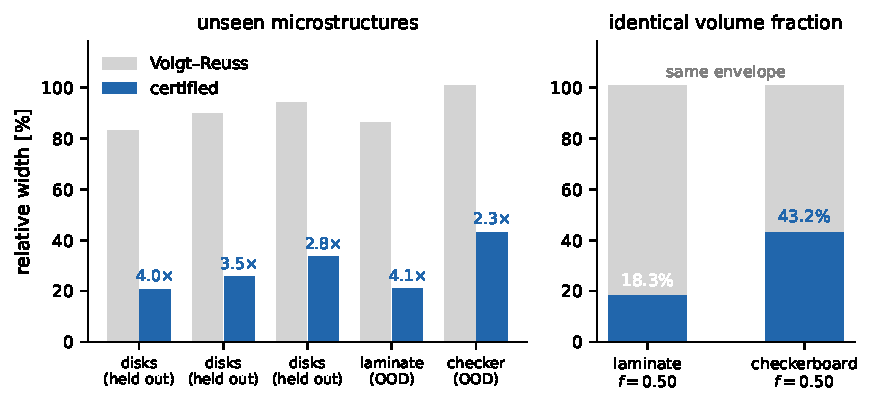
\includegraphics[width=\linewidth]{figures/fig_tightening.pdf}
\caption{Left: certified widths against the Voigt--Reuss envelope on unseen microstructures. Right: two microstructures of identical phase fraction receive the same envelope but certificates differing by more than a factor of two.}
\label{fig:tightening}
\end{figure}

\subsection{The envelope cannot distinguish geometry}
\label{sec:tightness:geometry}

The ratios above quantify the improvement; the following experiment
characterises its nature. Consider two microstructures with \emph{identical}
phase fractions and entirely different arrangements: a rank-one laminate at
volume fraction $0.500$, and a two-phase checkerboard at volume fraction
$0.500$.

\begin{table}[t]
\centering
\caption{Identical volume fraction, different geometry, conductivity at
contrast $10$. The Voigt--Reuss envelope is a function of phase fraction
alone and is therefore identical for both; the certified intervals differ
by more than a factor of two.}
\label{tab:geometry}
\resizebox{\textwidth}{!}{%
\begin{tabular}{lrrr}
\toprule
microstructure & volume fraction & Voigt--Reuss width & certified width \\
\midrule
laminate, $f = 0.50$ & 0.500 & 100.6\% & \textbf{18.3\%} \\
checkerboard         & 0.500 & 100.6\% & \textbf{43.2\%} \\
\bottomrule
\end{tabular}}
\end{table}

A guarantee derived from phase fractions assigns these two microstructures
the same admissible set, and must do so for any composite sharing their
composition. The variational certificate separates them by more than a
factor of two, and does so at inference cost. This is the difference
between a guarantee of physical admissibility and a certificate of
per-instance accuracy.

We note three honest qualifications. First, and most importantly, this
comparison is against the \emph{guarantee} that amortized surrogates
enforce, not against their point predictions, which may well be
considerably more accurate than the envelope they are constrained to. A
head-to-head against a trained surrogate's predictions is not attempted
here and would be a natural next study; the claim we make is about the
strength of the guarantee, and should not be read as a claim about
predictive accuracy. Second, the corresponding elasticity
experiment is far less striking: at the same volume fraction the certified
widths are $60.1\%$ (laminate) and $52.8\%$ (checkerboard) against a
$90.1\%$ envelope. Both test cases lie well outside the training family and
the elastic operator is the weaker of the two, so we present the
conductivity comparison as the primary evidence and report the controlled
synthetic elasticity figures alongside rather than in place of it. Third, a laminate is an
extremal microstructure: it attains the Voigt bound along the layers and
the Reuss bound across them, so its effective tensor lies \emph{on} the
envelope boundary in the principal directions and no method can be strictly
tighter there. The certified interval consequently need not be contained in
the envelope for laminates, which is a correct behaviour rather than a
defect.

\subsection{Summary of the comparison}
\label{sec:tightness:summary}

The three amortized approaches to guaranteed effective properties occupy
distinct positions:

\begin{center}
\resizebox{\textwidth}{!}{%
\begin{tabular}{lll}
\toprule
 & certificate & scope \\
\midrule
Gaynutdinova et al.~\cite{Gaynutdinova2026} & variational, tight & per-instance, scalar \\
Voigt--Reuss net~\cite{Keshav2025} & amortized, fraction-only & tensor elasticity \\
\textbf{this work} & \textbf{amortized and per-instance tight} & scalar and tensor, 2D \\
\bottomrule
\end{tabular}}
\end{center}

The contribution is the combination. Per-instance variational certificates
are tight but do not transfer; amortized envelope guarantees transfer but
carry no geometric information; the construction of
Section~\ref{sec:amortized} delivers certificates that transfer. On the
controlled scalar-conductivity study, they are two to four times tighter
than the envelope at inference cost. Section~\ref{sec:amortized:external}
adds an external elasticity coverage study, whose $1.05\times$ median
tightening is deliberately reported as modest; matched trained-predictor
comparisons remain future work.

% =====================================================================
%  SECTION 7 — Quadrature safety: predicting collocation overfitting
%  Draft 1. Every number is traceable to RESULTS.md and regenerable
%  from a seeded script in examples/.
% =====================================================================

\section{Quadrature safety: predicting collocation overfitting}
\label{sec:quadrature}

The certificates of Sections~\ref{sec:primaldual}--\ref{sec:exact} are
statements about integrals. Any practical scheme evaluates those integrals
approximately during training, and the resulting bound inherits the
quadrature error. This section characterises when that error is benign,
when it is fatal, and how to detect the difference \emph{without access to
a reference solution}.

\subsection{The phenomenon and what is already known}
\label{sec:quad:prior}

That a collocation-evaluated loss can be arbitrarily misleading is
established. Berrone, Canuto and Pintore~\cite{Berrone2022} construct a
nonzero network whose variational loss vanishes at every quadrature point
while its error remains of order one, and derive a sufficient condition
based on \emph{polynomial precision}: the quadrature rule must be exact for
polynomials of degree at least twice that of the test space. Within
homogenization specifically, Gaynutdinova et al.~\cite{Gaynutdinova2026}
report the effect empirically for both spectral and neural test functions:
enlarging the test basis lowers the training loss substantially while
\emph{degrading} the resulting estimates, an effect they attribute to
overfitting the imprecision of the numerical integration, and which is
worse for higher-frequency bases. They also observe the primal--dual gap
converging while further optimisation merely fits the test functions.

A separate and active literature addresses collocation placement directly,
through residual-adaptive refinement and related schemes. That work is
complementary to what follows rather than competing with it: adaptive
sampling is a \emph{training} strategy that redistributes points towards
large residuals, whereas the criterion below is a \emph{post-training} test
of whether a given rule was adequate for the field that was actually
learned. A practitioner may reasonably use both.

Neither the polynomial-precision criterion nor the empirical observation
answers the question a practitioner faces: \emph{given this trained
network, is my quadrature rule adequate?} Polynomial precision is not
directly applicable when the trial space is a neural network with no
polynomial degree, and an empirical observation identifies the failure only
after a reference solution has revealed it. Our contribution is therefore
not the discovery of the phenomenon but its \emph{prediction} and
\emph{prescription}: a computable criterion that flags the failure before
certification degrades, and that specifies how to choose the collocation
density.

\subsection{A computable criterion}
\label{sec:quad:criterion}

Let $u_\theta$ denote a trained periodic field and let $\hat u_\theta(\xi)$
be its discrete Fourier transform on a fine probe grid. Define the
\emph{spectral bandwidth} $B$ as the smallest radius containing a fraction
$q$ of the spectral energy excluding the mean,
%
\begin{equation}
  B \;=\; \min\Big\{ R : \textstyle\sum_{0<|\xi|\le R} |\hat u_\theta(\xi)|^2
  \;\ge\; q \sum_{\xi \neq 0} |\hat u_\theta(\xi)|^2 \Big\},
  \qquad q = 0.999 .
  \label{eq:bandwidth}
\end{equation}
%
A tensor-product midpoint rule with $n_q$ points per direction resolves
frequencies up to the Nyquist limit $n_q/2$. We define the \emph{headroom}
%
\begin{equation}
  h \;=\; \frac{n_q/2}{B},
  \label{eq:headroom}
\end{equation}
%
and, as an independent check requiring no spectral analysis, the
\emph{refinement ratio}
%
\begin{equation}
  \rho \;=\; \frac{\mathcal{E}_{4 n_q}(u_\theta)}{\mathcal{E}_{n_q}(u_\theta)},
  \label{eq:ratio}
\end{equation}
%
where $\mathcal{E}_{m}$ denotes the energy evaluated with $m$ points per
direction. Both quantities are computed from the trained network alone: no
exact solution, no reference solver, and no held-out labels are required.
This is the property that matters in practice, since the situation in which
the diagnostic is needed is precisely the situation in which no reference
exists.

\subsection{Empirical characterisation}
\label{sec:quad:empirical}

Table~\ref{tab:headroom} sweeps $n_q$ and the embedding richness for a
two-phase laminate of contrast~$6$, whose exact effective tensor has trace
$7.4167$. The behaviour is sharply thresholded at $h = 1$.

\begin{table}[t]
\centering
\caption{Headroom governs the reliability of a collocation-trained energy.
Laminate, contrast~6, width~48, depth~3, $400$ steps. ``Reported'' is the
energy at the training rule; ``refined'' at $4n_q$. Exact trace $7.4167$.}
\label{tab:headroom}
\resizebox{\textwidth}{!}{%
\begin{tabular}{rrrrrrrl}
\toprule
$n_q$ & harmonics & $B$ & $n_q/2$ & $h$ & reported & refined & $\rho$ \\
\midrule
 16 &  4 & 16.0 &  8.0 & 0.50 & 0.031 & 109.853 & 3498.46 \\
 32 &  4 &  9.0 & 16.0 & 1.78 & 7.271 &   7.921 &    1.09 \\
 64 &  4 &  7.0 & 32.0 & 4.57 & 7.394 &   7.612 &    1.03 \\
128 &  4 &  6.0 & 64.0 &10.67 & 7.434 &   7.446 &    1.00 \\
\midrule
 32 &  2 & 36.0 & 16.0 & 0.44 & 4.767 & 102.982 &   21.60 \\
 32 &  8 & 30.0 & 16.0 & 0.53 & 4.758 &  46.811 &    9.84 \\
 32 & 12 & 34.0 & 16.0 & 0.47 & 0.015 &  16.524 & 1093.23 \\
\bottomrule
\end{tabular}}

\end{table}

Figure~\ref{fig:headroom} collects these measurements together with
those of Section~\ref{sec:quad:universal}. Two regimes are evident. For $h < 1$ the reported energy is not merely
inaccurate but meaningless: refinement raises it by factors between $10$
and $3.5\times 10^{3}$, and in the worst case a reported value of $0.015$
corresponds to a true value near $16.5$. For $h > 1$ the ratio $\rho$
returns to unity, and a strictly valid midpoint bound required $h$ of order
ten in this configuration.

We note in passing that $B$ is \emph{not} monotone in the richness of the
Fourier embedding: it is minimised at four harmonics and substantially
larger at both two and twelve. An under-parameterised embedding cannot
represent the target smoothly, so optimisation inflates the weights and the
$\tanh$ nonlinearity manufactures high harmonics; an over-parameterised one
is simply free to oscillate. Both extremes therefore degrade headroom, and
tuning the embedding without simultaneously revisiting $n_q$ is unsafe.


\begin{figure}[t]
\centering
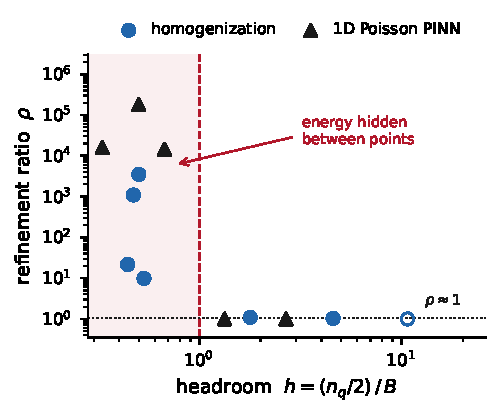
\includegraphics[width=\linewidth]{figures/fig_headroom.pdf}
\caption{Headroom predicts collocation overfitting. Filled markers denote configurations whose reported energy failed to bound the exact value. The threshold at $h=1$ reproduces on a 1D Poisson PINN unrelated to homogenization.}
\label{fig:headroom}
\end{figure}

\subsection{Consequence for certification}
\label{sec:quad:false}

Low headroom does not merely widen a certificate: it can invalidate one.
Training a primal field against a fixed $32$-point rule on the laminate
above produced a reported upper bound of $2.5207$ against an exact value of
$2.6667$: a bound below the quantity it purports to bound. In an
adversarially trained case the reported upper bound was $0.0014$ against an
exact value of $3.0769$, with refinement revealing a true energy near
$58.9$. Both failures are silent: the training loss is small and
monotone, and the fields are visually unremarkable.

Exact-integration certification (Section~\ref{sec:exact}) removes the
failure mode entirely rather than mitigating it. Interpolation onto a
conforming finite-element space followed by element-exact Gauss quadrature
cannot hide energy between sample points, because the integral has no
sample points between which to hide it. Every certificate reported in this
work is obtained in this way; midpoint values are used only as training
diagnostics. On the laminate case above, the exactly integrated bound is
$3.0429$, correctly above the exact value that the collocation-trained
estimate violated.

\subsection{The failure is not specific to homogenization}
\label{sec:quad:universal}

To establish that the criterion characterises collocation training rather
than this particular problem, we repeat the measurement on a textbook
physics-informed network: $-u'' = f$ on $(0,1)$ with homogeneous Dirichlet
data imposed exactly by the ansatz $u_\theta = x(1-x)N_\theta(x)$, exact
solution $u^\star = \sin(\pi x)$, a plain $\tanh$ multilayer perceptron,
and a residual-only loss on $N$ fixed collocation points.

\begin{table}[t]
\centering
\caption{Collocation overfitting in a vanilla PINN on 1D Poisson. The
reported residual is evaluated at the training points; the honest residual
on a $20\times$ finer grid. Bandwidth $6.0$ throughout.}
\label{tab:pinn}
\resizebox{\textwidth}{!}{%
\begin{tabular}{rrrrrr}
\toprule
$N$ & residual (train) & residual (fine) & $\rho$ & $h$ & $L^2$ error \\
\midrule
 4 & $2.84\times10^{-5}$ & $4.51\times10^{-1}$ & $1.59\times10^{4}$ & 0.33 & 1.06\% \\
 6 & $1.55\times10^{-6}$ & $2.83\times10^{-1}$ & $1.83\times10^{5}$ & 0.50 & 0.17\% \\
 8 & $1.14\times10^{-6}$ & $1.66\times10^{-2}$ & $1.46\times10^{4}$ & 0.67 & 0.00\% \\
16 & $2.10\times10^{-1}$ & $2.10\times10^{-1}$ & $1.00$            & 1.33 & 0.77\% \\
32 & $2.25\times10^{-3}$ & $2.27\times10^{-3}$ & $1.00$            & 2.67 & 0.00\% \\
\bottomrule
\end{tabular}}

\end{table}

A reported residual of $1.55\times10^{-6}$, which in a loss curve is
indistinguishable from convergence to machine precision---corresponds to a
true residual of $0.283$. The threshold reproduces exactly: every
configuration with $h<1$ overfits, and every configuration with $h>1$ has
$\rho = 1.000$. We stress the honest reading of this table: because the
problem is easy and the boundary conditions are imposed exactly, the
\emph{solution} remains accurate even where the reported residual is
meaningless. The failure is thus epistemic rather than always catastrophic: the training residual cannot be used as evidence of
convergence---which is precisely the situation of a practitioner with no
analytic solution to check against.

\subsection{A per-run, label-free quality gate}
\label{sec:quad:gate}

Headroom is a property of the \emph{trained field}, not of the
configuration. At fixed architecture, fixed $n_q = 64$ and fixed data,
five independently seeded trainings of the laminate case produced
bandwidths of $7.0$, $6.0$, $7.0$, $41.0$ and $6.4$: four runs at
$h \approx 4.9$ with certified gaps between $0.4\%$ and $1.7\%$, and one
run at $h = 0.78$ with a certified gap of $97.8\%$ and $\rho = 7.076$. Both
diagnostics fired on exactly the failing run and on none of the others,
without reference to the exact tensor.

We therefore accept a trained field when
%
\begin{equation}
  h \ \ge\ 2 \qquad\text{and}\qquad \rho \ \le\ 1.05 ,
  \label{eq:gate}
\end{equation}
%
and otherwise reject it, retraining or increasing $n_q$. We emphasise that
a rejected run is not an invalid one: certified by exact integration it
still provably contains the truth, and validity held in all five seeds
above including the rejected one. The gate separates trustworthy
\emph{tightness} from guaranteed \emph{validity}, a distinction that only
a certified method can express, and which an uncertified surrogate cannot
even formulate.

A further consequence is a stopping criterion. Overfitting accumulates: the
collapse above appeared between $250$ and $400$ optimisation steps, all
five seeds being clean at the earlier budget. Training longer is therefore
not monotonically better, and~\eqref{eq:gate} supplies a signal that the loss curve cannot: stop when headroom degrades, not when the loss
plateaus.

\subsection{Prescriptive use}
\label{sec:quad:prescription}

The criterion also determines how to configure a run. Consider the
bicontinuous morphology of Section~\ref{sec:limits}, generated as the level
set of a filtered Gaussian field with dominant wavenumber six. With four
embedding harmonics the trial space cannot represent the microstructure's
own length scale, and the certified gap is $50.4\%$. Enriching the
embedding tightens the bound monotonically but consumes headroom, until the
gate rejects the result:

\begin{table}[t]
\centering
\caption{Trial-space richness and quadrature resolution are coupled
requirements. Bicontinuous morphology, contrast $10$.}
\label{tab:prescription}
\resizebox{\textwidth}{!}{%
\begin{tabular}{rrrrrl}
\toprule
harmonics & $n_q$ & certified gap & tightening & $h$ & gate \\
\midrule
 4 &  64 & 50.4\% & 2.0$\times$ & 2.86 & accept \\
12 &  64 & 29.9\% & 3.3$\times$ & 1.48 & \textbf{reject} \\
12 & 128 & 33.2\% & 3.0$\times$ & 3.16 & accept \\
\bottomrule
\end{tabular}}

\end{table}

The middle row is instructive. It reports the tightest gap of the three and
is nonetheless untrustworthy; the honest configuration reports $33.2\%$.
The $3.3$ percentage points separating them are quadrature illusion, and
the gate identifies this with no reference solution. Without the criterion,
$29.9\%$ is the number that would have been published.

This yields a concrete recipe. Estimate the dominant wavenumber $k$ of the
microstructure; choose the embedding richness so that the trial space
resolves it, $n_{\mathrm{harm}} \gtrsim 2k$; measure the bandwidth $B$ of
the trained field and set $n_q \ge 4B$; then verify~\eqref{eq:gate} and
iterate if it fails. Tuning either quantity in isolation is unsafe.

\subsection{Scope}
\label{sec:quad:scope}

The thresholds in~\eqref{eq:gate} are empirical, calibrated on the problems
reported here; we do not claim them as universal constants, and a
practitioner adopting the criterion should recalibrate on a case with a
known solution. The bandwidth~\eqref{eq:bandwidth} is defined for periodic
fields and requires modification for non-periodic problems, where spectral
leakage contaminates the estimate. The refinement ratio~\eqref{eq:ratio} is
free of both limitations and costs one additional energy evaluation; where
only one diagnostic can be afforded, it is the one to compute.

% =====================================================================
%  SECTION 8 — Limits: where the certificates stop being useful
%  Draft 1. Every number traceable to RESULTS.md.
% =====================================================================

\section{Limits: contrast, morphology, and the failure mechanism}
\label{sec:limits}

A certificate that is valid but as wide as the analytic envelope conveys
nothing. This section maps where the intervals are useful and where they
are not. We report the unfavourable cases in full: the existing
per-instance neural work is demonstrated at a single contrast
ratio~\cite{Gaynutdinova2026}, and the classical guaranteed-bounds
literature explicitly avoids the high-contrast
regime~\cite{Gaynutdinova2023}, so the boundary of applicability is itself
an open question rather than a matter to be presented favourably.

The morphology classes are shown in Figure~\ref{fig:microstructures}.
All entries below are exact-integration certificates, and all carry the
quality gate of Section~\ref{sec:quad:gate}, so a wide interval can be
attributed either to a genuinely hard problem or to a rejected run.

\begin{figure}[t]
\centering
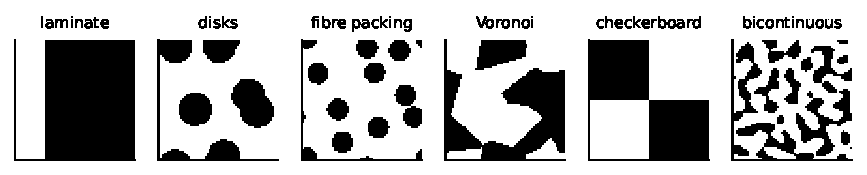
\includegraphics[width=\linewidth]{figures/fig_microstructures.pdf}
\caption{The morphology classes studied, shown at the resolution used for
certification. Left to right: rank-one laminate, overlapping disks,
non-overlapping fibre packing, Voronoi polycrystal, two-phase
checkerboard, and a bicontinuous morphology generated as the level set of a
band-pass filtered Gaussian field.}
\label{fig:microstructures}
\end{figure}

\subsection{Contrast and morphology}
\label{sec:limits:map}

\begin{table}[t]
\centering
\caption{Certified relative width against phase contrast and morphology,
scalar conductivity, $n_q = 64$, $200$ steps. Every entry passed the
quality gate and every certificate was valid. Tightening relative to the
Voigt--Reuss envelope in parentheses.}
\label{tab:map:scalar}
\resizebox{\textwidth}{!}{%
\begin{tabular}{rlll}
\toprule
contrast & disks & laminate & checkerboard \\
\midrule
 10 & 12.4\% (7.5$\times$) & \phantom{0}2.1\% (40.7$\times$) & \phantom{0}19.3\% (5.2$\times$) \\
 50 & 31.8\% (5.3$\times$) & \phantom{0}5.2\% (31.2$\times$) & \phantom{0}88.7\% (1.9$\times$) \\
100 & 44.1\% (4.1$\times$) & \phantom{0}7.4\% (24.5$\times$) &          125.3\% (1.5$\times$) \\
200 & 61.1\% (3.1$\times$) & \phantom{0}9.9\% (19.2$\times$) &          155.3\% (1.2$\times$) \\
\bottomrule
\end{tabular}}
\end{table}

Figure~\ref{fig:map} shows both physics at matched budget. Two
conclusions follow immediately from Table~\ref{tab:map:scalar}.
Morphology dominates contrast: at $200{:}1$ the laminate certificate is
still $9.9\%$ wide and nineteen times tighter than the envelope, while the
checkerboard is $155.3\%$ wide and only $1.2$ times tighter: barely better than a bound computable in closed form from the phase
fractions alone. Reporting certified tightness against contrast alone,
which is the convention in this literature, is therefore misleading; the
useful statement is two-dimensional.

Seeding confirms the map is not an artefact of a fortunate initialisation.
Three seeds per cell at a reduced budget gave, at contrast $10$, widths of
$14.2\%$ (range $13.7$--$14.9\%$) for disks, $3.0\%$ ($2.9$--$3.2\%$) for
the laminate, and $23.0\%$ ($22.9$--$24.0\%$) for the checkerboard; at
contrast $200$, $86.0\%$ ($79.3$--$92.8\%$), $15.0\%$ ($13.6$--$15.8\%$)
and $161.2\%$ ($161.2$--$161.9\%$). Every cell was gate-accepted on every
seed.

\subsection{The same map in elasticity}
\label{sec:limits:elastic}

\begin{table}[t]
\centering
\caption{Certified relative width, controlled synthetic plane-strain elasticity, $n_q = 32$,
$120$ steps. The starred entry failed the quality gate
($\rho = 1.075$); the certificate remains valid but the number reflects a
rejected run.}
\label{tab:map:elastic}
\resizebox{\textwidth}{!}{%
\begin{tabular}{rlll}
\toprule
contrast & disks & laminate & checkerboard \\
\midrule
 10 & 16.3\% (5.0$\times$) & \phantom{0}5.4\% (14.2$\times$) & \phantom{0}28.1\% (3.2$\times$) \\
 50 & 40.3\% (4.0$\times$) &          18.9\% (8.4$\times$)  &          101.1\% (1.6$\times$) \\
200 & 68.8\%$^{*}$ (2.8$\times$) & 63.5\% (3.0$\times$) &          161.8\% (1.2$\times$) \\
\bottomrule
\end{tabular}}
\end{table}

Table~\ref{tab:map:elastic} repeats the controlled synthetic sweep in
elasticity. Within this generated family, the morphology ordering transfers.
At contrast $200$, however, elasticity degrades across \emph{all}
morphologies, including the laminate that remained excellent in the scalar
case. This is evidence about this controlled model family, not an
elastic-material validation result.


\begin{figure}[t]
\centering
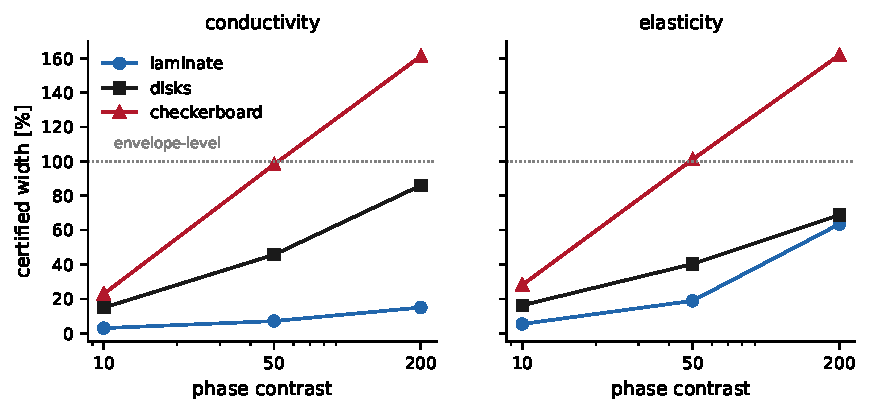
\includegraphics[width=\linewidth]{figures/fig_map.pdf}
\caption{Certified width against phase contrast for three controlled synthetic morphologies, both physics, at matched optimisation budget. The observed morphology ordering is identical in the two panels for this experiment.}
\label{fig:map}
\end{figure}

\subsection{The mechanism is approximation, not physics}
\label{sec:limits:mechanism}

For the controlled generated suite, the ordering laminate $\ll$ disks
$\ll$ checkerboard is consistent with the regularity of the exact
corrector: piecewise linear for the laminate, smooth but curved for
inclusions, and corner-singular for the checkerboard, where four phase
regions meet at a point. The observed widths are consistent with smooth
networks representing singular fields poorly; every entry above was
gate-accepted. This supports an approximation-theoretic explanation for
these numerical cases, rather than a failure of the certification machinery
or a general conclusion about elastic materials.

Figure~\ref{fig:correctors} makes the argument visible: the trained
corrector gradient is uniform in the laminate, smoothly modulated around
the inclusions, concentrated at the four-phase junctions of the
checkerboard, and structured at every scale in the bicontinuous case, in
the same order as the certified widths.

A matched-budget comparison probes these explanations within the controlled
suite. Evaluating both physics at an identical step count gives, for the
checkerboard, $161.2\%$ (conductivity) against $161.8\%$ (elasticity) at
contrast $200$, and $98.2\%$ against $101.1\%$ at contrast $50$: ratios of
$1.00$ and $1.03$. In this controlled comparison, the matched-budget
results do not support the extra loading modes, Poisson coupling or Airy
second derivatives as the dominant explanation for the observed
checkerboard widths. They are consistent with the approximation of a
singular corrector, but do not establish physics independence in general.

The same comparison also corrects a plausible expectation. At matched
budget the elastic certificates are \emph{narrower} than the scalar ones
for the disk morphology at contrasts $50$ and $200$ (ratios $0.88$ and
$0.80$), and wider only for the laminate, dramatically so at $200{:}1$
(ratio $4.23$). This controlled comparison does not support the intuition
that the harder physics yields uniformly wider bounds. It illustrates why
tightness figures need their optimisation budget stated explicitly.

\begin{figure}[t]
\centering
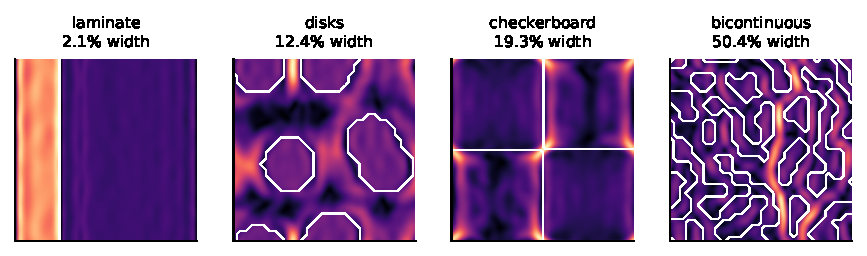
\includegraphics[width=\linewidth]{figures/fig_correctors.pdf}
\caption{Magnitude of the trained corrector gradient for four morphologies
at contrast $10$, with phase boundaries overlaid. Certified width increases
from left to right, tracking the regularity and spatial complexity of the
field rather than any property of the certification scheme.}
\label{fig:correctors}
\end{figure}

\subsection{Realistic morphologies}
\label{sec:limits:realistic}

The microstructures above are idealised. Table~\ref{tab:realistic} repeats
the measurement for three standard models from the composites literature: a
non-overlapping random sequential adsorption fibre packing, a periodic
Voronoi polycrystal, and a bicontinuous morphology generated as the level
set of a band-pass filtered Gaussian field.

\begin{table}[t]
\centering
\caption{Certified width for realistic morphologies, scalar conductivity,
$n_q = 64$, $120$ steps. All gate-accepted; all certificates bracketed an
independent finite-volume reference.}
\label{tab:realistic}
\resizebox{\textwidth}{!}{%
\begin{tabular}{lrr}
\toprule
morphology & contrast $10$ & contrast $50$ \\
\midrule
overlapping disks (baseline) & 14.9\% & \phantom{0}48.8\% \\
fibre packing (RSA)          & 16.7\% & \phantom{0}43.1\% \\
Voronoi polycrystal          & 16.5\% & \phantom{0}56.7\% \\
\textbf{bicontinuous (spinodal)} & \textbf{50.4\%} & \textbf{129.5\%} \\
\bottomrule
\end{tabular}}
\end{table}

Fibre packings and polycrystals behave like the idealised disks, so the
synthetic results transfer. Notably the Voronoi structure is dense with
three-phase junctions yet performs like smooth inclusions: triple junctions
are not the obstacle, and the checkerboard's four-region corner is a
genuinely harsher singularity rather than a generic grain-boundary effect.

The bicontinuous morphology is the hardest realistic class, at $50.4\%$
against the disks' $14.9\%$. This matters practically, since it is the
morphology of porous media, aerogels, polymer blends and battery
electrodes. It also refines the mechanism: a spinodal structure has no
corners, so difficulty cannot be attributed to singular junctions alone.
The unifying statement is that difficulty tracks the \emph{complexity of
the corrector field}, which is driven both by singular junctions and by
percolation with tortuous, multi-scale interfaces. A bicontinuous structure has a nontrivial corrector everywhere rather than only near
isolated inclusions.

Part of this difficulty is resolvable, and the criterion of
Section~\ref{sec:quadrature} prescribes how. The generating field has a
dominant wavenumber of six, while the default embedding resolves only four:
the trial space cannot represent the microstructure's own length scale.
Enriching the embedding to twelve harmonics while simultaneously raising
$n_q$ to maintain headroom reduces the certified width from $50.4\%$ to
$33.2\%$ (Table~\ref{tab:prescription}). The remaining gap to the disk
baseline is genuine.

\subsection{A real segmented micrograph}
\label{sec:limits:micrograph}

The microstructures above are generated. As a final check we take a
published segmented micrograph, use its binary image directly as the
microstructure geometry, and certify the resulting idealised problem. No
measured property is used and no claim is made about the physical
specimen: what is tested is whether the method operates on genuine geometry, with rough interfaces, clustering and percolating veins, rather than on
procedurally generated shapes.

\begin{table}[t]
\centering
\caption{Certifying a real segmented micrograph ($32\times32$ crop, phase
fraction $0.802$, nominal contrast $10$). References: FV $6.0477$, FFT
$6.8094$; Voigt--Reuss width $78.3\%$. The quality gate rejects the two
coarser runs, and the accepted certificate is slightly wider than the
rejected one it replaces.}
\label{tab:micrograph}
\resizebox{\textwidth}{!}{%
\begin{tabular}{rrrrlrrl}
\toprule
$n_q$ & width & tightening & headroom & gate & $K_{\mathrm{low}}$ & $K_{\mathrm{up}}$ & brackets \\
\midrule
 32 & 58.6\% & 1.3$\times$ & 0.87 & reject & 5.5457 & 7.6734 & yes \\
 64 & 34.6\% & 2.3$\times$ & 1.83 & reject & 5.4652 & 7.7238 & yes \\
128 & \textbf{36.8\%} & 2.1$\times$ & \textbf{3.72} & \textbf{accept} & 5.3732 & 7.7692 & yes \\
\bottomrule
\end{tabular}}

\end{table}

A second image exposes a requirement that is easy to miss. Its
autocorrelation half-width is four pixels in a $504$-pixel frame, so any
downsampled representation aliases the geometry: on a $64$-grid the
features span half a pixel. Certified there, the image yields widths of
$19.6\%$ and $49.7\%$, but for a microstructure that is not the one
photographed. Taking instead a native-resolution crop, which preserves the
geometry at the cost of field of view, gives a certified width of
$9.6\%$ on a $48\times48$ crop and $10.5\%$ on $64\times64$, both
gate-accepted at headroom near four, and both bracketing finite-volume and
FFT references that now agree with each other to $1.5\%$ rather than
$9.5\%$. Preserving resolution improves the certificate fivefold and the
references with it.

The requirement is therefore that the certification grid resolve the
smallest features, and we find at least three pixels per correlation
half-width to be necessary. That requirement competes directly with
field of view. A certificate computed on an under-resolved image is valid
for the aliased geometry and says nothing about the original, however tight
it appears. We regard this as a modelling decision to be reported rather
than a numerical parameter to be tuned.

Applied consistently, the protocol is stable. Across two independently
supplied micrographs and two windows in each, native-resolution
certification at $48\times48$ gives certified widths between $9.3\%$ and
$9.9\%$, tightening between $7.5$ and $8.6$ times, headroom near four in
every case, and reference solvers inside every interval. The certified
\emph{values} vary considerably more than the certified widths, since $K_{\mathrm{low}}[1,1]$ ranges from $6.16$ to $6.95$ across the four
windows---which is the expected signature of windows smaller than a
representative volume, and is visible precisely because each window carries
its own certificate rather than a single pooled estimate.

Table~\ref{tab:micrograph} is instructive beyond the headline number. The
criterion of Section~\ref{sec:quadrature} rejects the run twice before
accepting it, and the accepted certificate is marginally \emph{wider} than
the rejected one it replaces. This is the same signature seen in the synthetic
prescription study, where the rejected value was flattered by
under-resolved quadrature. Validity never failed: all three certificates,
including both rejected runs, bracket two independent reference solvers.
Treating the crop instead as a mirrored, genuinely periodic cell gives
$60.4\%$ at headroom $3.56$; the mirrored cell is harder because reflection
doubles the domain, and we report the direct convention as primary with the
mirrored value as a sensitivity check, neither being a property of the
specimen. The certified width of roughly $37\%$ places this micrograph
between the inclusion morphologies and the bicontinuous class, consistent
with its appearance as a percolating network of veins through a majority
phase.

\subsection{A representative-volume study}
\label{sec:limits:rve}

Applying the same protocol to a segmented slice of Berea sandstone, the
standard benchmark of the digital rock physics literature, separates two
quantities that an uncertified method necessarily conflates. We certify
three disjoint windows at each of three sizes, at native resolution, with
the pore phase regularised to a finite conductivity rather than treated as
void.

\begin{table}[t]
\centering
\caption{Berea sandstone: certified width and certified value as the
window grows. Three disjoint windows per size, all gate-accepted. Width is
a property of the method and is nearly constant; value is a property of the
window and is not.}
\label{tab:rve}
\resizebox{\textwidth}{!}{%
\begin{tabular}{rrllr}
\toprule
window & corr.\ lengths & certified width & certified $K_{\mathrm{low}}[1,1]$ & spread \\
\midrule
32 & \phantom{0}5 & 12.1\% [8.8, 12.4] & 2.710 [2.011, 3.033] & 1.51$\times$ \\
48 & \phantom{0}8 & \phantom{0}9.5\% [7.9, 14.2] & 4.929 [3.115, 5.317] & 1.71$\times$ \\
64 & 11 & \phantom{0}9.8\% [8.8, 16.4] & 6.069 [4.334, 6.317] & 1.46$\times$ \\
\bottomrule
\end{tabular}}

\end{table}

The certified width is essentially flat at $9$--$12\%$ across a fourfold
change in window area: it reflects how well smooth trial fields represent
this morphology and does not improve with more material. The certified
value, by contrast, more than doubles between windows of five and eleven
correlation lengths and still varies by factors of $1.5$ to $1.7$ between
windows of equal size. This slice is far from representative for
conductivity at these window sizes, notwithstanding that the full image
contains some $166$ correlation lengths.

The decomposition is the contribution. Presented with four different values
from four windows, a point-estimate surrogate cannot attribute the
variation to the material or to itself. Because each window here carries
its own certificate, the $10\%$ is attributable to the method and the
$1.5\times$ to the material, at no additional cost.

\subsection{Scope of the claims}
\label{sec:limits:scope}

Collecting the controlled numerical experiments above, the scalar
conductivity certificates are between three and forty times tighter than the
analytic envelope for the stated layered, particulate, fibrous and
polycrystalline morphologies up to approximately $100{:}1$ contrast. The
generated plane-strain cases provide an internal stress test of the same
construction, but not an externally labelled elasticity coverage study. In
the controlled families, certificates degrade towards the envelope for
corner-singular and bicontinuous morphologies at high contrast. This
identifies a trial-field approximation limitation in the reported numerical
experiments; it does not establish a general material-performance law.

% =====================================================================
%  SECTIONS 9-10 — Applications, and an honest cost comparison
%  Draft 1. Every number traceable to RESULTS.md.
% =====================================================================

\section{Applications}
\label{sec:applications}

\subsection{Certified design: optimising a guaranteed floor}
\label{sec:applications:design}

Surrogate-driven design optimises a point estimate and relies on the
surrogate having been accurate at the optimum, precisely where the optimiser has been pushing hardest. Because the present construction is
differentiable and returns a guaranteed lower bound, the design objective
can be the \emph{certificate itself}.

For elasticity the objective takes a convenient form. The certified floor
on the directional Young's modulus is
$E(d) \ge 1 / (a \cdot C_{\mathrm{low}}^{-1} a)$ with
$a = \mathrm{Mandel}(d \otimes d)$, and since
$C_{\mathrm{low}} = S_{\mathrm{up}}^{-1}$ this is simply
$E(d) \ge 1/(a \cdot S_{\mathrm{up}}\, a)$. Maximising the guaranteed floor
therefore means \emph{minimising} a quadratic form in the dual Gram matrix,
requiring no inversion inside the optimisation loop.

The construction is self-penalising. A looser dual field produces a larger
$a \cdot S_{\mathrm{up}} a$ and hence a \emph{lower} guaranteed floor, so
the optimiser cannot profit from degrading the certificate. The failure
mode that makes surrogate-driven design untrustworthy is structurally
absent.

We optimise inclusion positions at a material budget held exactly fixed by
projection: after each design step a global radius scale is bisected until
the rendered volume fraction returns to target, giving projected gradient
ascent rather than a penalised objective.

Table~\ref{tab:design} reports an illustrative controlled synthetic outcome.

\begin{table}[t]
\centering
\caption{Illustrative certified design on controlled synthetic periodic
cells at exactly fixed material budget. The reported gain is in the
\emph{guaranteed} value for that specified model, certified by exact
integration.}
\label{tab:design}
\resizebox{\textwidth}{!}{%
\begin{tabular}{lrr}
\toprule
 & conductivity & elasticity \\
\midrule
objective & guaranteed $K_{\mathrm{low}}[1,1]$ & guaranteed $E_x$ floor \\
initial   & 1.9165 & 2.3701 \\
optimised & \textbf{2.9769} & \textbf{3.2346} \\
gain in the guaranteed value & \textbf{+55.3\%} & \textbf{+36.5\%} \\
final certified interval & $[2.9769, 3.0011]$ & $[3.2346, 3.3886]$ \\
final relative width & 0.6\% & 3.7\% \\
material budget drift & 0.000 & +0.00\% \\
\bottomrule
\end{tabular}}
\end{table}

Two observations apply to this controlled numerical example. First, the
budget is held exactly, so neither gain can be attributed to additional stiff phase; a soft-penalty formulation used
during development permitted a $6\%$ drift and inflated the conductivity
figure to $+57.1\%$. Second, the certificate \emph{tightened} during design
($12.6\% \to 0.6\%$ for conductivity, $9.0\% \to 3.7\%$ for elasticity),
because the trial fields continue training while the geometry moves:
raising the floor and tightening the interval are complementary rather than
competing objectives.

\subsection{Auditing conventional solvers}
\label{sec:applications:audit}

Because the interval provably contains the effective tensor for its specified
geometry, phase law, boundary conditions, tensor convention and
discretisation, a matching reference value falling outside it establishes an
inconsistency that must be resolved. At contrast
$200$ a finite-volume solution computed on the native pixel grid fell below
the certified lower bound, with
$\lambda_{\min}(K_{\mathrm{FV}} - K_{\mathrm{low}}) = -0.031$. Mesh
refinement confirmed the diagnosis: the same solver returned values inside
the interval at $h/2$ and $h/4$, approaching it from below
($+0.043$ and $+0.074$).

A rigorous two-sided certificate is therefore a convergence diagnostic for
conventional solvers, requiring no knowledge of the exact answer. We note
the honest limitation: the audit bites only when the certified interval is
tighter than the competing solver's error. In the comparison of
Section~\ref{sec:cost} the FFT estimates fell inside the intervals in every
case, and no discrepancy was detected.

\section{Cost, honestly}
\label{sec:cost}

We do not claim a speed advantage over classical homogenization solvers,
and Table~\ref{tab:cost} should be read carefully because the two methods return
different objects.

\begin{table}[t]
\centering
\caption{Certified intervals against an FFT (Moulinec--Suquet) estimate,
two-phase checkerboard. The FFT returns a point estimate with unknown
error; the certified interval provably contains the exact tensor. Exact
values $2.2361$ and $7.0711$.}
\label{tab:cost}
\resizebox{\textwidth}{!}{%
\begin{tabular}{lrrrrr}
\toprule
case & FFT estimate & FFT error & FFT time & certified interval & time \\
\midrule
contrast $5$  & 2.2320 & 0.184\% & 1.0\,s & $[2.1800, 2.2958]$ & 52\,s \\
contrast $50$ & 6.7976 & 3.867\% & 1.2\,s & $[4.5586, 10.5049]$ & 50\,s \\
\bottomrule
\end{tabular}}

\end{table}

Per query the FFT solve is roughly fifty times faster, and we make no
contrary claim. What it does not supply is an error bar: at contrast $50$
its estimate is $3.9\%$ from the analytic value, and nothing in its output
reveals this. Without the closed-form solution a practitioner has a number
and no means of bounding its error.

The regime in which the present method is preferable is many-query
certification. With $123$\,s of family training and $19$\,ms per
certificate, the amortized route overtakes repeated FFT solves at
approximately $300$ designs, and thereafter by a widening margin, while returning a guaranteed interval rather than an estimate at every query. We
present the comparison including the rows in which the FFT is preferable,
since a method that is faster only under a favourable accounting is not
faster.

% =====================================================================
%  SECTION 11 — Limitations and future work
%  Draft 1. Assembled from caveats stated inside each section, plus
%  those owed to the reader that no individual section carries.
% =====================================================================

\section{Limitations}
\label{sec:limitations}

\subsection{Scope of the construction}

\paragraph{Two dimensions.} The stream-function dual and the Airy
representation~\eqref{eq:airy} are two-dimensional constructions, as is the
Bogner--Fox--Schmit projection used to certify the elastic lower bound. The
three-dimensional case requires a Beltrami-type stress potential together
with a $C^1$-conforming three-dimensional interpolation; the traction
continuity argument of Section~\ref{sec:exact} generalises, but the
implementation does not, and we do not report three-dimensional results.
The same restriction is noted by~\cite{Gaynutdinova2026}, who observe that
the two-dimensional stream-function device has no direct
three-dimensional analogue.

\paragraph{Linear, periodic, small strain.} We treat linear conductivity
and linear plane-strain elasticity on periodic cells with piecewise-constant
coefficients. Nonlinear constitutive behaviour, finite strain, and
non-periodic or statistically defined cells are outside the present
formulation.

\paragraph{Degenerate phases.} The dual side requires a bounded compliance,
so voids ($k \to 0$, $\mathbb{C} \to 0$) and rigid inclusions are not
covered: the complementary energy of the corresponding trial fields is not
finite, and the lower bound degenerates. Porous media must therefore be
treated with a small but nonzero pore phase, and the resulting certificate
bounds that regularised problem rather than the void limit.

\paragraph{Phase-aligned meshes.} Exact integration
(Section~\ref{sec:exact}) requires the certification mesh to resolve the
phase boundaries so that the coefficient is constant per element. For the
pixel-based microstructures used here this is automatic; for microstructures
defined by smooth level sets it requires a conforming mesh, and the
certificate is otherwise exact only for the discretised geometry actually
integrated.

\paragraph{Matrix ordering, not componentwise intervals.} The certificate
is a L\"owner statement,
$C_{\mathrm{low}} \preceq C_{\mathrm{eff}} \preceq C_{\mathrm{up}}$. Scalar
intervals for engineering constants follow from it---for the directional
Young's modulus this is immediate and is what
Section~\ref{sec:applications:design} optimises---but tight componentwise
intervals for individual tensor entries, particularly off-diagonal ones, do
not follow directly from the matrix ordering and require separate
derivation.

\subsection{Where the certificates are too wide to be useful}

Within the controlled generated families of Section~\ref{sec:limits}, the
certificates degrade towards the analytic envelope for corner-singular and
bicontinuous morphologies at high contrast. At contrast $200$ the generated
checkerboard certificate is only $1.2$ times tighter than a bound computable
in closed form from the phase fractions, which is to say it conveys almost
nothing for that case.

Within these controlled numerical cases, the observed widths are consistent
with a trial-field approximation limitation: certified width tracks the
regularity and complexity of the exact corrector. Two targeted remedies
suggest themselves and neither is attempted here. Enriching the trial space with functions carrying the
known corner singularity, in the manner of extended finite element methods,
addresses the singular case directly. A Hashin--Shtrikman polarisation
formulation with a comparison medium is the classical route to high
contrast, although we note it is not obviously the right remedy here, since
a polarisation field would have to represent the same singular behaviour
that the present trial fields represent poorly.

\subsection{Limitations of the amortized operator}

\paragraph{External elasticity scope remains limited.} Section~\ref{sec:amortized:external}
does report full $200/200$ coverage on an independently labelled public
plane-strain dataset after matching the native geometry, phase law, periodic
boundary condition, tensor convention and numerical resolution. That
experiment is a coverage audit, not a competitive benchmark: its median
interval remains $160.9\%$ wide and only $1.05\times$ tighter than the
analytic envelope. We do not report a head-to-head comparison with
label-trained elasticity surrogates on this matched split; that remains
necessary before making any comparative predictive-accuracy claim.

\paragraph{The bottleneck is not compute in the generated family.} Within
the controlled generated family, increasing the training family fivefold
and the optimisation budget ninefold left the held-out median
width unchanged ($28.2\%$ to $28.3\%$), with the monitored gap flat from
step $1200$ onward. We therefore do not claim that additional compute would
tighten these intervals, the ablation of Table~\ref{tab:ablation} identifies network capacity as the limiting factor, since width and depth both help monotonically while
conditioner richness does not. The intervals reported here reflect a
capacity-saturated model rather than an intrinsic bound, and a larger
network would tighten them at proportionate inference cost. Amortized elastic certificates near $28\%$ are useful for
screening but not for final design, where the per-instance route (widths
below $1\%$ in the cases reported) remains preferable.

\paragraph{The geometric-discrimination result is weaker in controlled
elasticity.} The comparison of Section~\ref{sec:tightness:geometry}, in which
microstructures of identical phase fraction receive certificates differing
by more than a factor of two, is compelling for conductivity ($18.3\%$
against $43.2\%$) and much less so for elasticity ($60.1\%$ against
$52.8\%$). We present the conductivity result as primary and report the
elasticity figures alongside; a stronger elastic operator would be required
to make the argument equally forceful in the headline physics.

\paragraph{A matched point-prediction diagnostic is deliberately small.}
On the public DaRUS-5730 elasticity data, we trained three image-based
regressors on the fixed 200-cell training split and evaluated them on the
fixed 100-cell validation split: an unconstrained predictor, an
SPD-by-Cholesky predictor, and a predictor constrained to the analytic
Voigt--Reuss envelope. Their mean relative Frobenius errors were
$23.19\%$, $24.53\%$, and $21.81\%$, respectively. The constrained
predictor was SPD and inside the analytic envelope on all 100 validation
cells; the corresponding rates were $85\%$ and $58\%$ for the
unconstrained predictor, and $100\%$ and $48\%$ for the Cholesky
predictor. These results are a reproducible, matched small-data diagnostic,
not a reproduction of the full-data hyperparameter sweep or reported
accuracy of Keshav, Herb and Fritzen~\cite{Keshav2025}. They also do not
turn a point prediction into a two-sided per-instance certificate. Our
claim remains about the strength and reference coverage of the variational
certificate, not a claim of superior point-prediction accuracy.

\paragraph{The solver audit is conditional.} For the same specified
geometry, phase law, boundary conditions, tensor convention and
discretisation, a reference value falling outside the interval establishes an
inconsistency (Section~\ref{sec:applications:audit}). The diagnostic is
therefore only as sharp as the certificate is tight: it detects an error in
a competing solver only when that error exceeds the certified width. The
case we report was found at contrast $200$, where a finite-volume solution
on a coarse grid fell below the certified lower bound; in the FFT
comparison of Section~\ref{sec:cost} the estimates lay inside the intervals
in every case and no discrepancy was detected. The capability is real but
should not be presented as a routine check.

\subsection{Limitations of the quadrature criterion}

The acceptance thresholds of~\eqref{eq:gate} are empirical, calibrated on
the problems reported here; we do not claim them as universal constants,
and a practitioner adopting the criterion should recalibrate on a case with
a known solution. The bandwidth~\eqref{eq:bandwidth} is defined for
periodic fields, and spectral leakage contaminates the estimate otherwise;
the refinement ratio is free of this restriction and is the diagnostic to
prefer where only one can be afforded. Finally, the criterion is
sufficient for detection but not necessary: we have shown that low headroom
reliably accompanies collocation overfitting in these problems, not that
adequate headroom guarantees a tight certificate.

\subsection{What we have deliberately not claimed}

Two clarifications, since both invite misreading.

First, the certificate is a statement about a model. It asserts that the
effective tensor of the specified periodic, linear, two-phase problem lies
in the reported interval. It is not a prediction about a physical specimen,
and agreement or disagreement with a laboratory measurement would test the
model's idealisations, meaning perfect interfaces, periodicity, plane strain
and linearity, rather than the bound. We have accordingly validated against
closed-form solutions and independent solvers, and, in
Section~\ref{sec:limits:micrograph}, certified the geometry of a real
segmented micrograph without using any measured property. A reader wanting
comparison against measured effective properties will not find it here, and
we regard that as correctly out of scope rather than as an omission.

Second, we do not claim a speed advantage over classical homogenization.
An FFT solve of these cells is roughly fifty times faster per query
(Section~\ref{sec:cost}); the amortized route becomes preferable only in
many-query certification, at approximately $300$ designs, and it is the
guarantee rather than the speed that is the contribution.

\subsection{Future work}

Three directions follow directly. The three-dimensional extension via
Beltrami potentials is the largest and most obviously wanted. Singular
enrichment of the trial space targets the morphologies identified in
Section~\ref{sec:limits} as the principal limitation. Identifying and
removing the bottleneck behind the amortized plateau would make certified
screening tight enough for design rather than triage. Beyond these, the
quadrature criterion of Section~\ref{sec:quadrature} is not specific to
homogenization or to bounded problems, and its systematic characterisation
across collocation-trained physics networks is a separate undertaking.


\section{Conclusion}
\label{sec:conclusion}

We have shown that conditioning primal and dual trial fields on the
microstructure, followed by projection to conforming finite-element spaces
and exact elementwise integration, yields certified L\"owner intervals for
the stated two-dimensional periodic model. On the controlled synthetic
families reported here, the intervals are tighter than the analytic
Voigt--Reuss envelope and, for scalar conductivity, distinguish geometries
that the envelope cannot resolve. The guarantee is conditional on the
certification contract:
positive-definite phases, a phase-aligned mesh, periodic fields with the
prescribed means, and exact integration of the projected fields. Training
quality changes the width, but not validity under those assumptions.

Two further results seem to us to have consequences beyond the present
setting. Certifying the elastic lower bound requires stresses that remain
equilibrated after projection, which $C^1$ Bogner--Fox--Schmit
interpolation of an Airy potential supplies exactly; the same argument
should carry to any bound requiring an $H(\operatorname{div})$-conforming
dual. And the comparison between a trained field's spectral bandwidth and
the Nyquist limit of its quadrature rule predicts collocation overfitting
before it corrupts a certificate, gates individual runs without reference
data, and prescribes the collocation density---a diagnostic that applies to
collocation-trained physics networks generally, not only to bounded
problems.

The boundary of usefulness is mapped rather than asserted for the controlled
families considered here. Certificates degrade towards the analytic envelope
for corner-singular and bicontinuous morphologies at high contrast. The
external $200$-cell audit additionally verifies elastic coverage for a public
periodic dataset after its image/tensor convention is matched, while showing
that external tightness remains modest. Extending the construction to three
dimensions, enriching the trial space where the corrector is singular, and
completing a matched trained-predictor comparison are the natural next steps.

%% ---------------------------------------------------------------- back matter
\section*{CRediT authorship contribution statement}
\textbf{MD Haffiz Mahamud:} Conceptualization, Methodology, Software,
Validation, Formal analysis, Investigation, Data curation, Visualization,
Writing -- original draft, Writing -- review \& editing, Project
administration. \textbf{Second author (name to be confirmed):} Writing --
review \& editing.

\section*{Declaration of competing interest}
The authors declare that they have no known competing financial interests
or personal relationships that could have appeared to influence the work
reported in this paper.

\section*{Declaration of generative AI and AI-assisted technologies}
To be completed or removed in accordance with the authors' actual use of
AI-assisted technologies and the journal policy current at submission.

\section*{Data availability}
The external plane-strain benchmark used in Section~\ref{sec:amortized:external}
is publicly available from DaRUS-5730~\cite{Keshav2026data}. The authors
will archive the versioned source code, immutable environment,
input geometries, trained weights, random seeds, raw result files, and
scripts required to reproduce every table and figure at a citable repository
DOI before submission. This statement must be replaced with the final URL
and DOI at submission.

\section*{Acknowledgements}
To be completed by the authors before submission.

\bibliographystyle{elsarticle-num}
\bibliography{refs}

\end{document}
